\ProvidesPackage{commands}
\documentclass[11pt]{article}
\usepackage{epstopdf}
\usepackage{subfigure,graphicx}
\usepackage{amsmath}
\usepackage{epsf}
\usepackage{amsfonts}
\usepackage{amssymb}
\usepackage{color}
\usepackage{mathtools}
\usepackage{placeins}
\usepackage{booktabs}
\usepackage{enumitem}
\usepackage{caption}
\usepackage[margin=0.8in, paperwidth=8.5in, paperheight=11in]{geometry}
\usepackage{amsfonts}
\usepackage{amsmath}
\usepackage{amsbsy}
\usepackage{authblk}
\usepackage{graphicx}
\usepackage{listings}
\usepackage{array}
\usepackage{titlesec}
\usepackage{amssymb}
\usepackage{bm}
\usepackage{mathtools}
\usepackage{titlesec}

\usepackage[latin1]{inputenc}\newcommand{\bs}[1]{\boldsymbol{#1}}
\newcommand{\del}[2]{\frac{\partial {#1}}{\partial {#2}}}
\newcommand{\D}[2]{\frac{D^{\overline{\alpha}}}{\overline{\alpha !}}{#1}(#2,#2)\ {\bf x}^{\overline{\alpha}}}
\newcommand{\dv}[3]{\frac{{\rm d}^{#1}{#2}}{d{#3}^{#1}}}
\newcommand{\ddel}[5]{\frac{\partial^{ {#1} + {#2}} {#3}}{\partial {#4}^{#1} \partial{#5}^{#2}}}
\newcommand{\dev}{{\rm {\bf dev}}}
\newcommand{\proj}[1]{\frac{1}{R^2}{\bf X}\otimes{\bf X}}
\newcommand{\Ie}[1]{I^{\rm e}_{#1}}
\newcommand{\Ce}[1]{\bf C^{\rm e^{#1}}}
\newcommand{\Fe}[2]{F^{\rm e^{#2}}_{#1}}
\newcommand{\Fv}[2]{F^{\rm v^{#2}}_{#1}}
\newcommand{\f}[2]{f^{\rm {#2}}_{#1}}
\newcommand{\B}[2]{B^{\rm {#2}}_{#1}}
\newcommand{\E}[2]{E^{\rm {#2}}_{#1}}
\newcommand{\fv}[2]{f^{\rm v^{#2}}_{#1}}
\newcommand{\dfv}[2]{\dot{f}^{\rm v^{#2}}_{#1}}
\newcommand{\tGam}[2]{\tilde{\Gamma}^{\rm v^{#2}}_{#1}}
\newcommand{\Gam}[2]{\Gamma^{\rm v^{#2}}_{#1}}
\newcommand{\A}[1]{\mathcal{A}_{#1}}
\newcommand{\F}[2]{F^{\rm #2}_{#1}}
\newcommand{\hpeq}{\hat{\psi}^{\rm Eq}}
\newcommand{\hpneq}{\hat{\psi}^{\rm NEq}}
\newcommand{\etak}{\eta_K({I_1,I_2,J},{\bf C^{\rm e}, B^{\rm v}})}
\newcommand{\nuk}{\nu_K({I_1,I_2,J},{\bf C^{\rm e}, B^{\rm v}})}
\newcommand{\thetak}{\theta_K({I_1,I_2,J},{\bf C^{\rm e}, B^{\rm v}})}
\newcommand{\etaj}{\eta_J({I_1,I_2,J},{\bf C^{\rm e}, B^{\rm v}})}
\newcommand{\dFv}[2]{\dot{F}^{\rm v^{#2}}_{#1}}
\newcommand{\hatpsi}{\widehat{\psi}(I_1, I_2,I^{\rm e}_1,I^{\rm e}_2,J)}
\newcommand{\hpsi}{\widehat{\psi}(I_1,I^{\rm e}_1,J)}
\newcommand{\Fh}[1]{\widehat{\mathcal{F}}\left({\bf F, \Fv{}{}}, {#1}\right)}
\newcommand{\Fhstar}[1]{\widehat{\mathcal{F}}^*\left({\bf F, \Fv{}{}}, {#1}\right)}
\newcommand{\sbar}{\overline{\bm{\sigma}}}
\newcommand{\hpsicomp}[1]{\sum_{r=1}^{2}\left\{\frac{3^{1-\alpha_r}}{2\alpha_r}\mu_r(I^{\alpha_r}_1-3^{\alpha_r})
+\frac{3^{1-a_r}}{2a_r}m_r({\Ie{1}}^{^{a_r}}-3^{a_r})\right\}
+\mu{#1}+\kappa{#1}^2}
\newcommand{\Ni}[1]{N^{(e)}_i(#1)}
\newcommand{\hNi}[1]{\hat{{N}}^{(e)}_i(#1)}
\newcommand{\Ld}{L^{\dagger}}
\newcommand{\intinfinf}{\int_{-\infty}^{\infty} \int_{-\infty}^{\infty}}
\newcommand{\LLnorm}[1]{\left\lVert{#1}\right\rVert_2}
\newcommand{\Linorm}[1]{{\left\lVert{#1}\right\rVert_\infty}}
\newcommand{\tr}{\rm tr}
\newcommand{\deldel}[2]{\frac{\partial^2 {#1}}{\partial {#2}^2}}
\newcommand{\kd}[1]{\delta_{#1}}
\newcommand{\Fie}[1]{{\bf F}^{#1}}
\newcommand{\Comp}{\emph{CompStrainStress\_Cee570.m}}
\newcommand{\Comps}{\emph{CompStrainStress\_Elem\_Cee570.m}}
\newcommand{\Feap}{\emph{FEA\_Program.m}}
\newcommand{\Elast}{\emph{Elast2d\_Elem.m}}
\newcommand{\Assem}{\em{AssemStifForc.m}}
\newcommand{\Fb}{\em{F\_bar\_int}}
\newcommand{\Form}{\em{FormFE.m}}
\newcommand{\Sol}{\em{SolveFE.m}}
\newcommand{\inpt}{\em{triangtwo.m}}

\titlespacing\section{10pt}{10pt plus 4pt minus 2pt}{10pt plus 2pt minus 2pt}
\titlespacing\subsection{0pt}{8pt plus 4pt minus 2pt}{8pt plus 2pt minus 2pt}
\titlespacing\subsubsection{0pt}{12pt plus 4pt minus 2pt}{6pt plus 2pt minus 2pt}
\titlespacing*{\title}{-2ex}{*-2ex}{-2ex}
\usepackage{color} %red, green, blue, yellow, cyan, magenta, black, white
\definecolor{mygreen}{RGB}{28,172,0} % color values Red, Green, Blue
\definecolor{mylilas}{RGB}{170,55,241}
\setlength\parindent{0pt}
\graphicspath{{Figures/}}

\usepackage{graphicx}
\title{\bf CEE 576: Nonlinear Finite Elements \\ HW5}
\author{Bhavesh Shrimali \\ NetID: bshrima2}
\date{\today}
\begin{document}
\maketitle \hrule \hrule \hrule
\section*{Sol$^n$ 1: Average Acceleration Method}
From the class lecture: (Ignoring the damping effects as in the class-lecture, i.e. , ${\bf C} = \bf 0$)
\begin{itemize}
\item For the linear case the equilibrium equation is given by 
\begin{align*}
{\bf M}{\bf a}_{n+1} + {\bf K}{\bf d}_{n+1} = (1+\alpha){\bf F}_{n+1} - \alpha {\bf F}_n
\end{align*}
\item For the nonlinear case: 
\begin{align*}
{\bf M}{\bf a}_{n+1} = (1+\alpha)({\bf F}^{\rm ext}_{n+1} - {\bf N}({\bf d}_{n+1})) - \alpha ({\bf F}^{\rm ext}_n - {\bf N}({\bf d}_n))
\end{align*}
\end{itemize}
For the predictor multi-corrector algorithm:
\begin{align*}
{\bf a}^{i+1}_{n+1} & = {\bf a}^{i}_{n+1} + {\Delta}{\bf a} \\ \\
{\bf d}^{i+1}_{n+1} & = {\bf d}^{i}_{n+1} + {\Delta}{\bf d} \\ \\
& = {\bf d}^{i}_{n+1} + {\beta \Delta t^2}{ \Delta\bf a}
\end{align*}
We linearize the internal force vector about the state ${\bf N}({\bf d}^i_{n+1})$
\begin{align*}
{\bf N}({\bf d}^{i+1}_{n+1})
=
{\bf N}({\bf d}^{i}_{n+1})
+ \del{{\bf N}}{\bf d} ({\bf d}^{i}_{n+1}) \cdot {\beta\Delta t ^2 \Delta {\bf a}}
\end{align*}
The second term on the RHS is nothing but the consistent tangent. For the present case, we restrict our focus on the first order taylor-expansion and ignore the higher order term. Thus we have
\begin{align*}
{\bf M}{\bf \Delta \bf a}
+
{\bf K}(1+\alpha)\beta \Delta t^2 \Delta{\bf a}
=
(1+\alpha)({\bf F}^{\rm ext}_{n+1} - {\bf N}({\bf d}^i_{n+1})) - \alpha ({\bf F}^{\rm ext}_n - {\bf N}({\bf d}_n)) - {\bf M} {\bf a}^{i}_{n+1}
\end{align*}
Thus rearranging the terms we finally get 
\begin{align}
\boxed {
\left( {\bf M}
+
(1+\alpha)\beta \Delta t^2 {\bf K} \right){\Delta \bf a}
=
(1+\alpha){\bf F}^{\rm ext}_{n+1} - \alpha{\bf F}^{\rm ext}_n - [(1+\alpha){\bf N}({\bf d}^i_{n+1}) - \alpha {\bf N}({\bf d}_n)] - {\bf M} {\bf a}^{i}_{n+1}
}
\end{align}
Substituting, for the case of the average acceleration method, i.e., $\beta = 1/4$ and $\gamma = 1/2$ we get
\begin{align*}
\boxed {
\left( {\bf M}
+
(1+\alpha)\frac{1}{4} \Delta t^2 {\bf K} \right){\Delta \bf a}
=
(1+\alpha){\bf F}^{\rm ext}_{n+1} - \alpha{\bf F}^{\rm ext}_n - [(1+\alpha){\bf N}({\bf d}^i_{n+1}) - \alpha {\bf N}({\bf d}_n)] - {\bf M} {\bf a}^{i}_{n+1}
}
\end{align*}\newpage
\section*{Sol$^n$ 2: Energy Conserving Algorithm}
\begin{itemize}
\item Since for the trapezoidal rule, the energy conservation is violated in the long run, we make use of the principle of energy conservation and by defining an incremental energy functional. 
\item The nonlinear algebraic problem is reformulated as the Euler-Lagrange equation of the associated functional. The constraint equation is then enforced by employing the method of Lagrange-multiplier. 
\end{itemize}
For the predictor multi-corrector algorithm we have
\begin{align}
{\bf M}{\bf a}^{i+1}_{n+1} 
= 
(1+\alpha)({\bf F}^{\rm ext}_{n+1} - {\bf N}({\bf d}^{i+1}_{n+1})) - \alpha ({\bf F}^{\rm ext}_n - {\bf N}({\bf d}_n))
\label{Sol2}
\end{align} 
Also for the predictor-multicorrector algorithm, the internal force can be linearized as follows
\begin{align*}
{\bf N}({\bf d}^{i+1}_{n+1})
=
{\bf N}({\bf d}^{i}_{n+1})
+ \del{{\bf N}}{\bf d} ({\bf d}^{i}_{n+1}) \cdot {\beta\Delta t ^2 \Delta {\bf a}}
\end{align*}
The recurrence relations for the predictor corrector approach are as follows
\begin{align}
\begin{split}
\tilde{\bf d}_{n+1}
& =
{\bf d}_n + \Delta t {\bf v}_n + \left(\frac{1-2\beta}{2}\right){\Delta t}^2 {\bf a}_n \\
\tilde{\bf v}_{n+1}
& =
{\bf v}_n
+ \Delta t (1-\gamma){\bf a}_{n} \\
{\bf d}^{}_{n+1} 
& =  \tilde{\bf d}_{n+1}
+ \beta {\Delta t}^2 {\bf a}_{n+1} \\
{\bf v}^{}_{n+1}
& =
\tilde{\bf v}_{n+1} + \gamma \Delta t {\bf a}_{n+1}
\end{split}
\label{dn+1tilda}
\end{align}
From equation (\ref{Sol2}) we proceed further, using the finite-difference relations, for predictors, defined in equation (\ref{dn+1tilda}). All the quantities are converted to a single unknown, i.e., ${\bf d}_{n+1}$. 
\begin{align*}
{\bf d}_{n+1} 
& =
{\bf d}_n + \Delta t {\bf v}_n + \left(\frac{1-2\beta}{2}\right){\Delta t}^2 {\bf a}_n + \beta \Delta t^2 {\bf a}_{n+1}\\
{\bf v}^{}_{n+1}
& =
\tilde{\bf v}_{n+1} + \gamma \Delta t {\bf a}^{}_{n+1}\\
& = 
{\bf v}_n + \Delta t ((1-\gamma){\bf a}_n + \gamma {\bf a}_{n+1}) 
\end{align*}
We make use of $\beta = 1/4$ and $\gamma = 1/2$
\begin{align*}
{\bf d}_{n+1}
& =
{\bf d}_n + \Delta t {\bf v}_n + \left(\frac{1}{4}\right){\Delta t}^2 {\bf a}_n + \frac{1}{4}\Delta t^2 {\bf a}_{n+1} =  {\bf d}_n + \Delta t {\bf v}_n + \left( \frac{{\bf a}_n}{4}\right)\Delta t^2 + \frac{1}{4}\Delta t^2 {\bf a}_{n+1} 
\end{align*}
Substituting ${\bf a}_{n+1}$ in terms of ${\bf d}_{n+1}$ and other terms we get
\begin{align}
\begin{split}
{\bf a}_{n+1}
& =
\frac{4}{\Delta t^2}
\left({\bf d}_{n+1} - {\bf d}_{n} - \Delta t {\bf v}_n - \frac{\Delta t^2}{4}{\bf a}_n 
\right) \\
& =
-\left(
{\bf a}_n + \frac{4}{\Delta t}{\bf v}_n + \frac{4}{\Delta t^2}{\bf d}_n
\right) + \frac{4}{\Delta t^2} {\bf d}_{n+1}
\end{split}
\label{an+1}
\end{align}
We substitute equation (\ref{an+1})$_2$ into (\ref{Sol2}) and rewrite all the quantities in the predictor-multicorrector form to get
\begin{align*}
-{\bf M}\left(
{\bf a}_n + \frac{4}{\Delta t}{\bf v}_n + \frac{4}{\Delta t^2}{\bf d}_n
\right) 
+
\frac{4{\bf M}}{\Delta t^2}{\bf d}^{i+1}_{n+1}
= 
(1+\alpha)({\bf F}^{\rm ext}_{n+1} - {\bf N}({\bf d}^{i+1}_{n+1})) - \alpha ({\bf F}^{\rm ext}_n - {\bf N}({\bf d}_n)) \\
\implies 
\frac{4{\bf M}}{\Delta t^2}{\bf d}^{i+1}_{n+1}
=
{\bf M}\left(
{\bf a}_n + \frac{4}{\Delta t}{\bf v}_n + \frac{4}{\Delta t^2}{\bf d}_n
\right) 
+
(1+\alpha)({\bf F}^{\rm ext}_{n+1} - {\bf N}({\bf d}^{i+1}_{n+1})) - \alpha ({\bf F}^{\rm ext}_n - {\bf N}({\bf d}_n)) 
\end{align*}
The corresponding functional is therefore given by (multiplying by a virtual displacement $\delta d^{i+1}_{n+1}$ and integrating) 
\begin{align*}
\boxed{
\begin{aligned}
\mathcal{F} \left({\bf d}^{i+1}_{n+1}\right)
= {\bf d}^{{i+1}^T}_{n+1}\ 
\left(\frac{2{\bf M}}{\Delta t^2}\right)\  
{\bf d}^{i+1}_{n+1}
- 
{\bf d}^{{i+1}^T}_{n+1}
\left(
{\bf M}\left(
{\bf a}_n + \frac{4}{\Delta t}{\bf v}_n + \frac{4}{\Delta t^2}{\bf d}_n
\right) 
+
(1+\alpha)({\bf F}^{\rm ext}_{n+1}) \right. \\
\left. - \alpha ({\bf F}^{\rm ext}_n - {\bf N}({\bf d}_n))\right)
 - (1+\alpha)\ {\mathcal{U}}({\bf d}^{i+1}_{n+1})
\end{aligned}
}
\end{align*}
Similarly we rewrite the energy associated with the system at the time steps $t_n$ and $t_{n+1}$ as follows:
\begin{align*}
E_{n+1} = E_n 
+ 
\frac{1}{2}{({\bf d}_{n+1} - {\bf d}_n )}^T \left( {\bf F}^{\rm ext}_n + {\bf F}_{n+1} \right)
\end{align*}
where again
\begin{align*}
E_{n} 
=
\frac{1}{2}{\bf v}^T_n\ {\bf M}\ {\bf v}_n + {\mathcal{U}} ({\bf d}_n)
\end{align*}
We define the following
\begin{align*}
\mathcal{G}({\bf d}_{n+1})
=
E_{n+1} - E_n 
- \left( 
\frac{1}{2}{({\bf d}_{n+1} - {\bf d}_n )}^T \left( {\bf F}^{\rm ext}_n + {\bf F}_{n+1} \right)
\right)
\end{align*}
Also
\begin{align*}
\del{E_{n+1}}{{\bf d}_{n+1}}
=
\frac{2}{\Delta t}
{\bf M}
{\bf v}_{n+1}
+ 
{\bf N}({\bf d}_{n+1})
\end{align*}
and therefore
\begin{align*}
\del{\mathcal{G}}{{\bf d}_{n+1}}
=
\frac{2}{\Delta t}
{\bf M}
{\bf v}_{n+1}
+ 
{\bf N}({\bf d}_{n+1})
-\frac{1}{2}({\bf F}^{\rm ext}_{n+1}+{\bf F}^{\rm ext}_{n})
\end{align*}
We now cast the whole problem variationally
\begin{align*}
\mathcal{H}
({\bf d}_{n+1})
=
\mathcal{F}({\bf d}_{n+1}) + \lambda \mathcal{G}({\bf d}_{n+1})
\end{align*}
Taking variation with respect to ${\bf d}_{n+1}$ and $\lambda$
\begin{align*}
\delta \mathcal{H}
({\bf d}_{n+1}) = \left(\del{\mathcal{F}}{{\bf d}_{n+1}} 
+
 \lambda_{n+1} \del{\mathcal{G}}{{\bf d}_{n+1}}\right) \cdot \delta {\bf d}_{n+1}
+ \delta \lambda \mathcal{G}({\bf d}_{n+1}) = 0
\end{align*}
Therefore the euler-lagrange equations, in the predictor-multicorrector context, are given by 
\begin{align}
\nonumber \boxed{
\begin{aligned}
& \left( 
\frac{4{\bf M}}{\Delta t^2}{\bf d}^{i+1}_{n+1}
- \left(
{\bf M}\left(
{\bf a}_n + \frac{4}{\Delta t}{\bf v}_n + \frac{4}{\Delta t^2}{\bf d}_n
\right) 
+
(1+\alpha)({\bf F}^{\rm ext}_{n+1} - {\bf N}({\bf d}^{i+1}_{n+1})) - \alpha ({\bf F}^{\rm ext}_n - {\bf N}({\bf d}_n)) 
\right)
\right) \cdot {\delta {\bf d}_{n+1}}\\
& + \lambda^{i+1}_{n+1}  \left( 
\frac{2}{\Delta t}
{\bf M}
{\bf v}^{i+1}_{n+1}
+ 
{\bf N}({\bf d}^{i+1}_{n+1})
-\frac{1}{2}({\bf F}^{\rm ext}_{n+1}+{\bf F}^{\rm ext}_{n})
\right) \cdot {\delta {\bf d}_{n+1}} = 0\ \ \ \ \forall {\delta \bf d}_{n+1}
\end{aligned}
}
\end{align}
and
\begin{align*}
\boxed{
\delta \lambda \mathcal{G}({\bf d}_{n+1})=0 \ \ \ \ \ \forall \delta\lambda
}
\end{align*}
The above system of equations can be rewritten compactly in a matrix form, after consistent linearization with respect to ${\bf d}^{i+1}_{n+1}$, i.e., $\left({\bf d}^{i+1}_{n+1} = {{\bf d}^{i}_{n+1}} + {\Delta {\bf d}}\right)$ and $\left({\lambda}^{i+1}_{n+1} = {\lambda}^{i}_{n} + \Delta \lambda\right)$, to get  
\begin{align}
\begin{bmatrix}
{\bf A}_{11} & {\bf A}_{12} \\
{\bf A}_{21} & {\bf 0}
\end{bmatrix}
\begin{Bmatrix}
\Delta {\bf d}\\
\Delta \lambda
\end{Bmatrix}
=
\begin{bmatrix}
{\bf b}_1\\
{\bf b}_2
\end{bmatrix}
\label{AXB}
\end{align}
where 
\begin{align*}
{\bf A}_{11}
& =
(1+\lambda^i_{n+1})\frac{4\bf M}{\Delta t^2} + (1+\alpha) {\bf K}({\bf d}^i_{n+1}) + \lambda^i_{n+1} {\bf K}({\bf d}^i_{n+1}) =
\boxed{ 
(1+\lambda^i_{n+1}) \left( \frac{4\bf M}{\Delta t^2}\right)
+ (1+\alpha+\lambda^i_{n+1}) {\bf K}({\bf d}^i_{n+1})} \\
{\bf A}_{12}
& =\boxed{
\left( \frac{4\bf M}{\Delta t^2}\right) ({\bf d}^i_{n+1} - {\bf d}_n)
+
{\bf N}({\bf d}^i_{n+1})
-\left( \frac{2\bf M}{\Delta t}\right){\bf v}_n - \frac{1}{2} (\bf \F{n+1}{ext}-\F{n}{ext})}\\
{\bf A}_{21} 
& =
\boxed{\frac{2}{\Delta t} \left(
\left(
-{\bf v}_n + \frac{2}{\Delta t} \left( {\bf \dis{n+1}{i} - \dis{n}{}}
\right)
\right)^T {\bf M}
\right)
-\frac{1}{2}\left({\bf \F{n+1}{ext} + \F{n}{ext}}\right)^T + {\bf N}^T\left({\bf \dis{n+1}{i}}\right)
=
{\bf A}^T_{12}}\\
{\bf b}^i_1
& = \boxed{
\begin{aligned}
& \left(
1+\alpha + \frac{\lambda^i_{n+1}}{2}
\right)
{\bf\F{n+1}{ext}} 
- \left( 
\alpha -\frac{\lambda^i_{n+1}}{2}
\right)
{\bf \F{n}{ext}} 
- \alpha 
\left( 
{\bf N}
\left(
{\bf \dis{n+1}{i}}
\right)
-
{\bf N}
\left(
{\bf \dis{n}{}}
\right)
\right)
\\ 
& + 
\frac{4{\bf M}{\bf v}_n}{\Delta t} 
\left(
1+\frac{\lambda^i_{n+1}}{2}
\right)
+
{\bf M}{\bf a}_n
-
\left(
1+\lambda^i_{n+1}
\right) \left[
{\bf N}
\left(
{\bf \dis{n+1}{i}}
\right)
+
\frac{4{\bf M}}{\Delta t^2}
\left(
{\bf \dis{n+1}{i} - \dis{n}{}}
\right)
\right]
\end{aligned}
}\\
{\bf b}^i_{2}
& =
\boxed{
E_n
-
E^i_{n+1}
+ \frac{1}{2}
\left({\bf \dis{n+1}{i} - \dis{n}{}}\right)
\left(
{\bf \F{n+1}{ext} + \F{n}{ext}}
\right)
}
\end{align*}
\hrule \hrule \hrule
\section*{Finite Element Code Development:}
The Nonlinear FEM Code for the generalized alpha method with energy conservation is built on the existing code. Certain features, elaborating the beginning of the algorithm are as follows: 
\begin{itemize}
\item At the first load step ($n=0$) the quantities either known to us or initialized are as follows: (Note that ${\bf d}_X$ denotes the unconstrained displacements)
\begin{itemize}
\item $\lambda = 0$; $\Delta\lambda = 0$; ${\bf d}_X =$ given; 
\item $\dot{\bf d}_X = \bf 0$ (the initial velocity is given to be equal to zero)
\item ${\bf a}_0 = - {\bf M}_{dd}^{-1} {\bf N}({\bf \dis{\it X}{}})$, i.e., the acceleration of the system is calculated from the original equation of motion. 
\end{itemize}
\item Now for the first load step, which is nothing but the initial time $t_0$, we take the prescribed displacement and run one pass of the algorithm. This gives us the internal force, and the external force for that load step, i.e., corresponding ${\bf d}^{0}_1 = {\bf d}_{0}$. The corresponding displacement velocity and displacement are stored as the last converged value for this load step. 
\item We now move to the second load step and its first iteration. We start by defining the predictors, i.e., $\tilde{\bf d}_{n+1}$ and $\tilde{\bf v}_{n+1}$. We pull these predictors into the FEA Program and solve the linear system given in the equation (\ref{AXB}). 
\item The residual obtained in the very first iteration is designated as the zeroth residual ${\bf Res}_o$ to be used for checking convergence in all the succeeding iterations. 
\item The correctors are obtained after determining the solution of the linear system, given in (\ref{AXB}).  
 \item The iterations are continued, till the convergence criteria is satisfied or if the maximum number of iterations are reached. 
 \item If the convergence check is satisfied, the algorithm moves to the next load step in the Newton Raphson. 
\end{itemize}
\section*{Results: }
The corresponding plots, obtained for the displacement and the stresses, for a time step $(\Delta t) = 0.01s$ are given below. Note that the expression for body force used: (${\bf F}_{b_x} = 0.1\sin t$) \\ \hrule
\subsection*{Newmark Method ($\alpha = 0$ )}
The results obtained for the case when no body force is applied are as follows: 
\begin{itemize}
\item {\bf Displacement and Energy Time-Histories}
\begin{center}
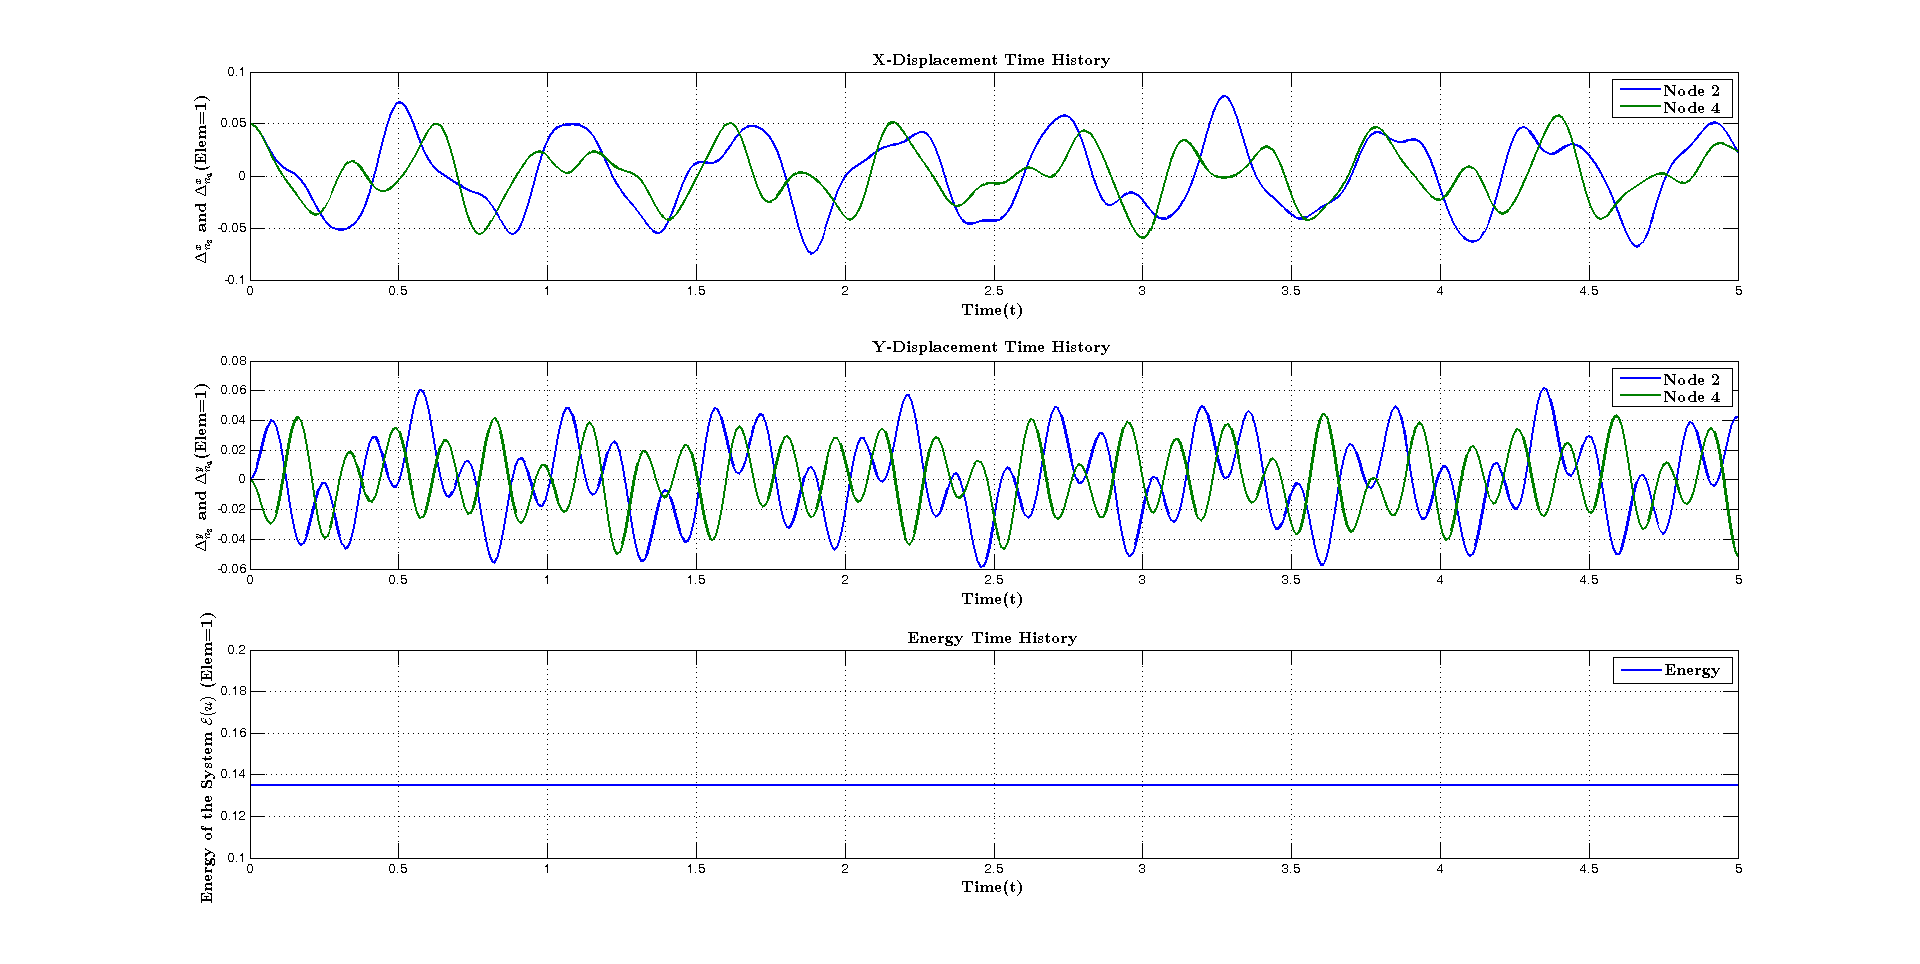
\includegraphics[height=5.5in,width=7in]{Disp_nobf_alphz}
\end{center}\hrule
\item { \bf Comments: } As a whole, the generalized alpha method, implemented for the given energy functional, conserves the energy. The displacement time-histories for the nodes 2 and 4 should not exactly be the same due to the slight difference in the boundary conditions in both the directions at the left edge of the problem (and hence the significant difference in phase and slight difference in the magnitude of the peak values). This is verified by the plots. 
\newpage 
\item {\bf Stress-Strain Time Histories}
\begin{center}
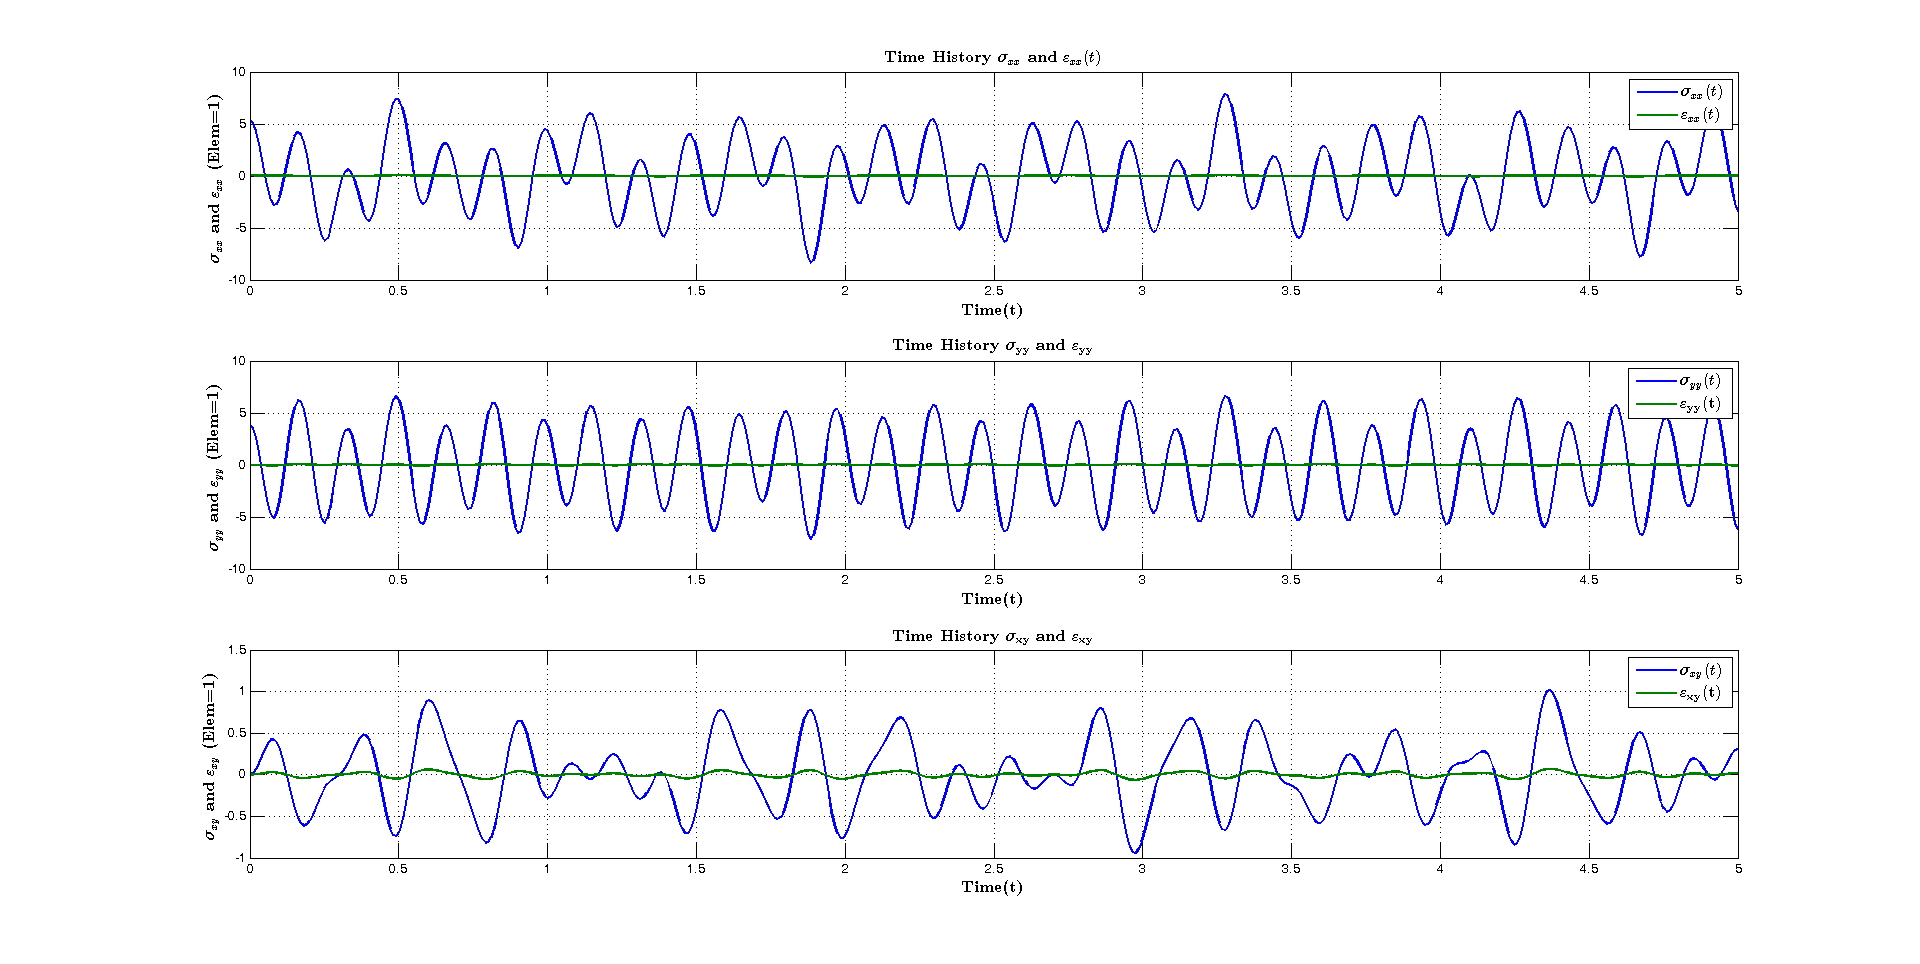
\includegraphics[height=5.5in,width=7in]{Stress_nobf_alphzer}
\end{center}\hrule
\item { \bf Comments: } The strains are typically small as the problem is restricted to small strain behavior. The stresses in the above analysis are determined based on the stored energy functional ($\partial W/\partial{\bm\varepsilon}$) and not on linearized calculation ($\bf D\cdot\varepsilon$). Though, for small strain calculations the stresses obtained from the stored energy functional can be linearized properly such that they agree with the linearized calculation. Since the external applied force is zero, it can be seen that the area under the stress-time diagram for one loading cycle is zero. Note that the area under the stress-time diagram would represent the change in the external traction force per unit length, for that time period, for a 2D mesh. (and hence should be equal to zero)    
\end{itemize}
\newpage The results obtained for the case when body force is applied are as follows: 
\begin{itemize}
\item {\bf Displacement and Energy Time-Histories}
\begin{center}
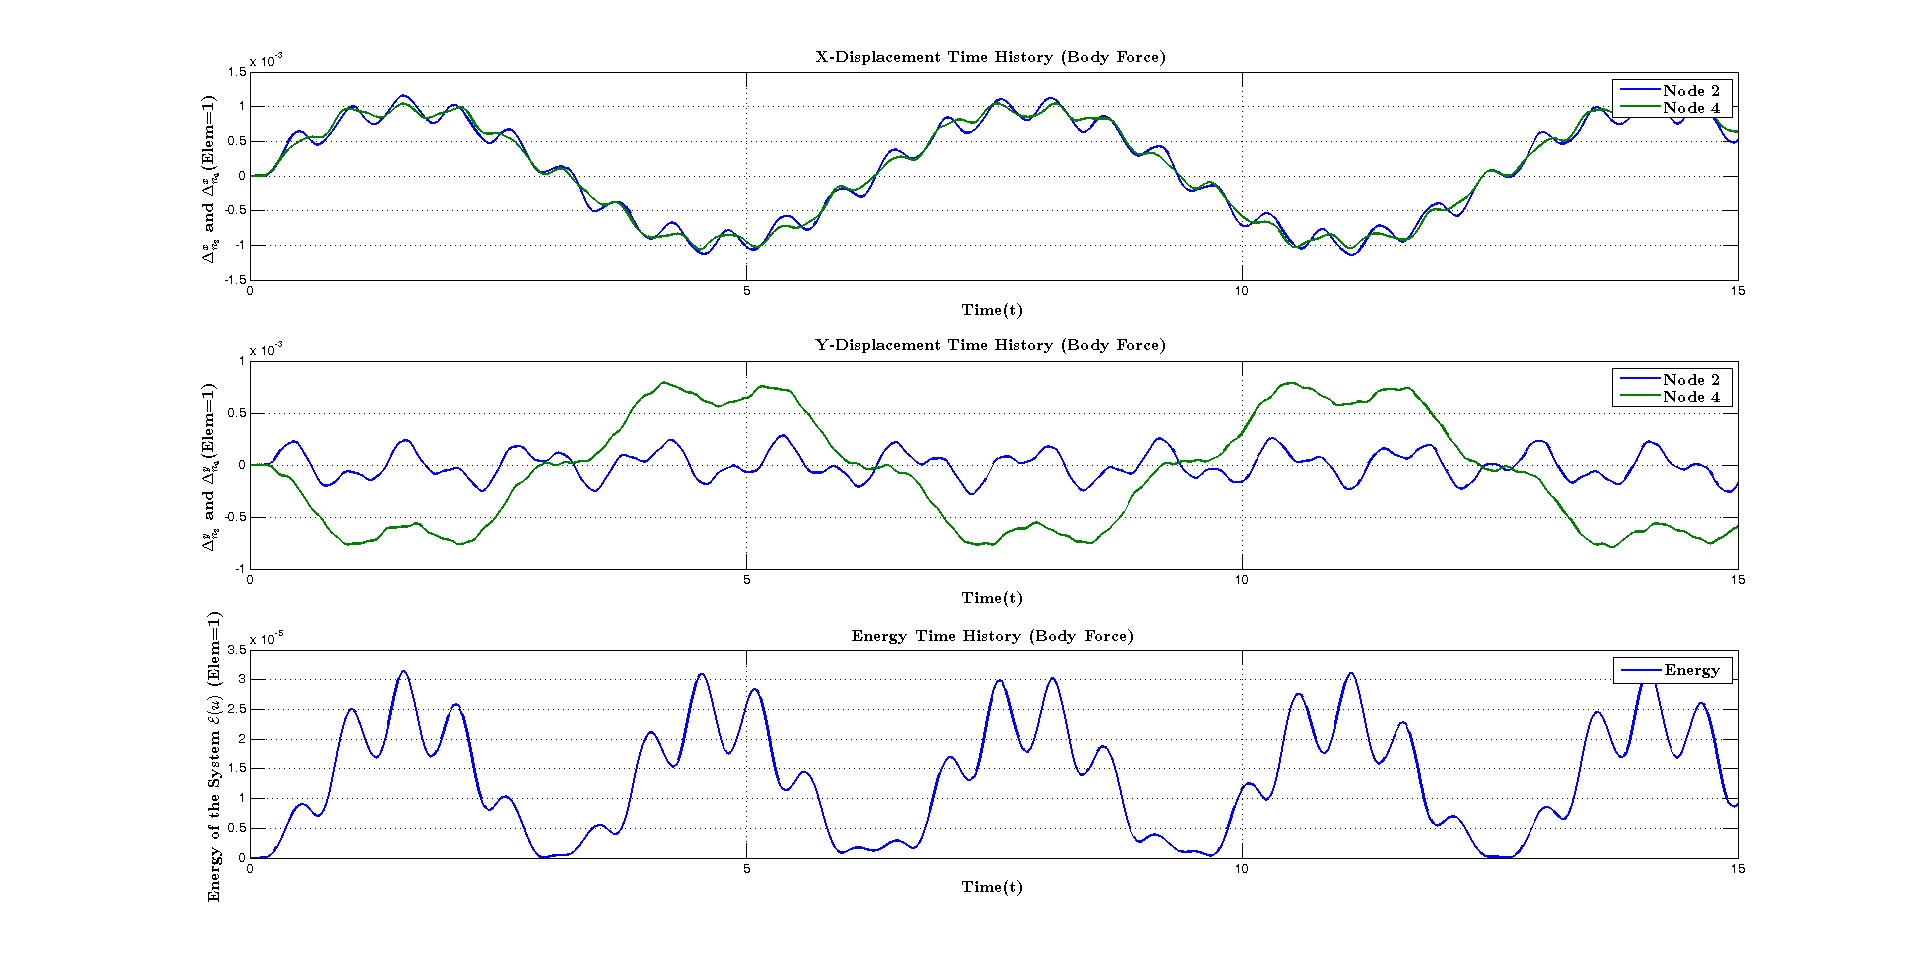
\includegraphics[height=5.5in,width=7in]{Disp_bf_alphz}
\end{center}\hrule
\item {\bf Comments:} Again nodes 2 and 4 have similar response, as in the previous case. Qualitatively, the higher response for node 4 in the y direction can be attributed to the boundary conditions at node 3 (since it is restricted to move only in x and not y direction.) The mean value of the energy in one cycle is nonzero. This can be attributed to the fact that we now have a body force prescribed in the problem statement as opposed to previously. Also the corresponding cycle-time ({\bf fundamental period}) is higher than the case when no body force was prescribed. 
\newpage 
\item {\bf Stress-Strain Time Histories}
\begin{center}
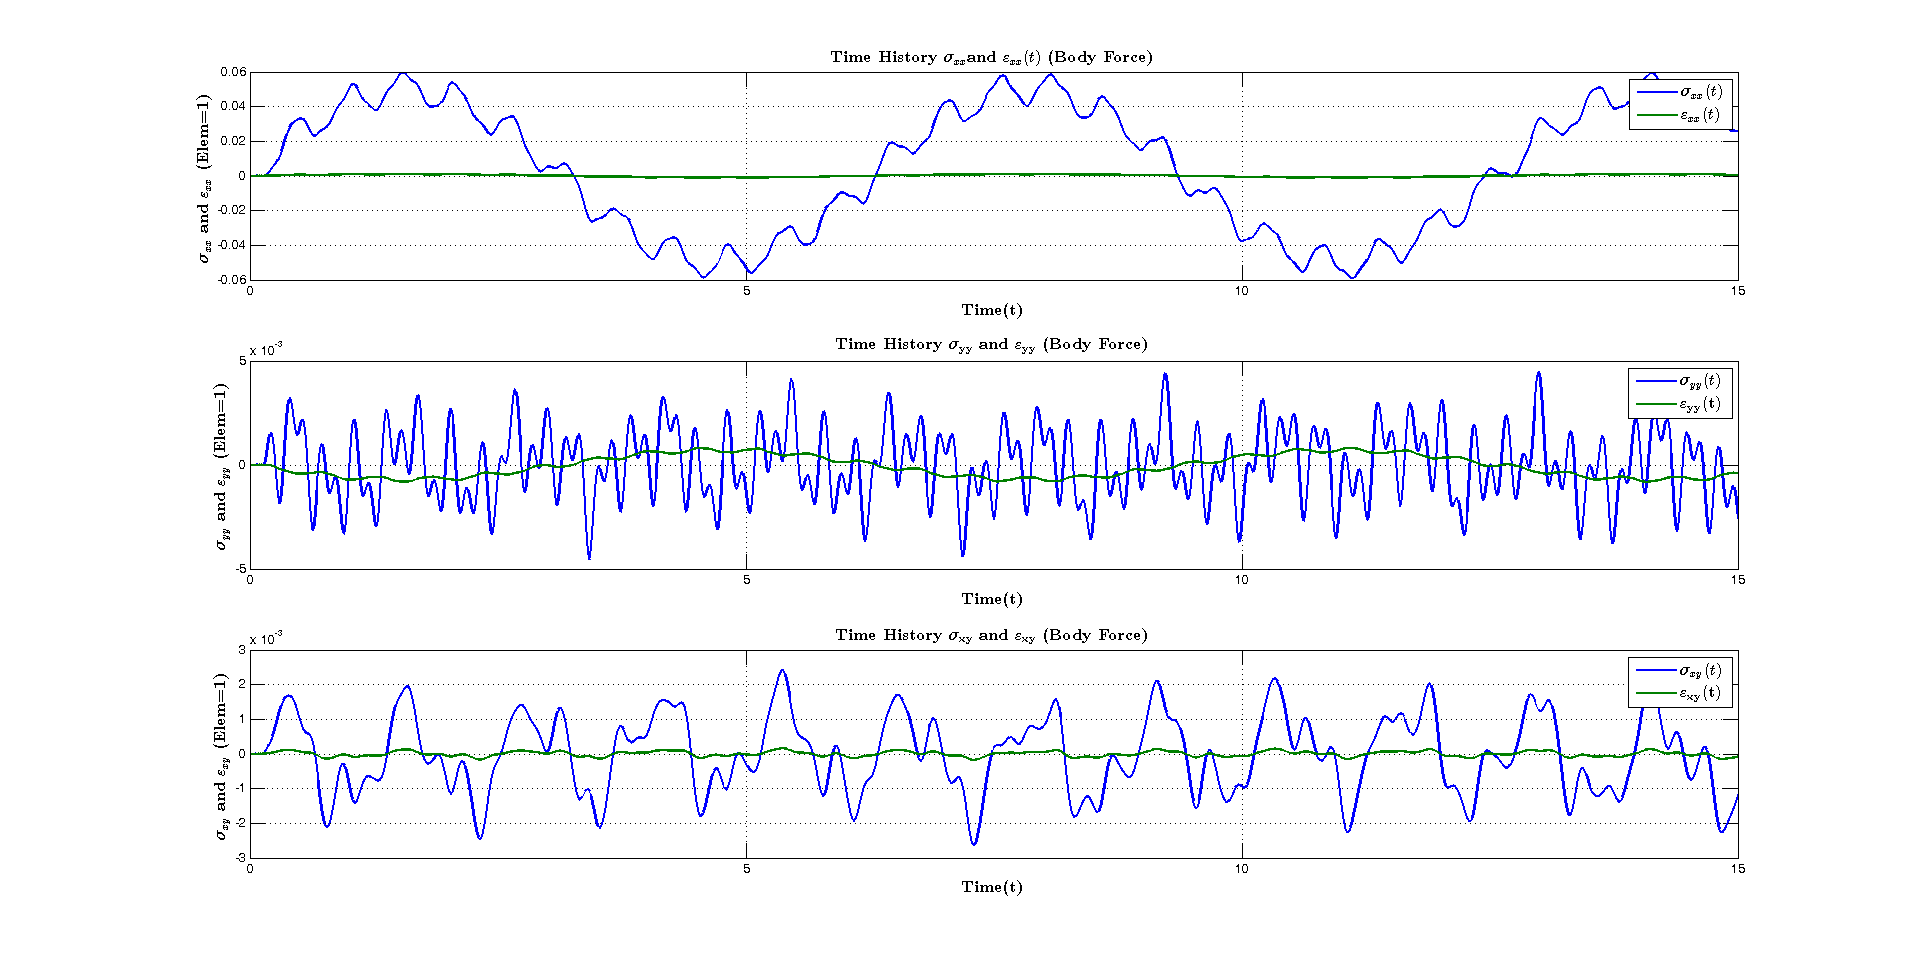
\includegraphics[height=5.5in,width=7in]{Stress_bf_alphz}
\end{center}\hrule
\item {\bf Comments: } It is worthwhile noting that the shear stresses are significantly lower than the  corresponding axial stresses. This is attributed to the nature of the problem as it is primarily axial. (theoretically it is exactly a uniaxial stress).
\end{itemize}
\newpage \subsection*{Case of ($\bm\alpha\bf = -\frac{1}{3}$ )}
The results obtained when no body force is applied are as follows: 
\begin{itemize}
\item {\bf Displacement and Energy Time-Histories} Note that the damping phenomena below can be circumvented using a lower time increment ($\Delta t$)
\begin{center}
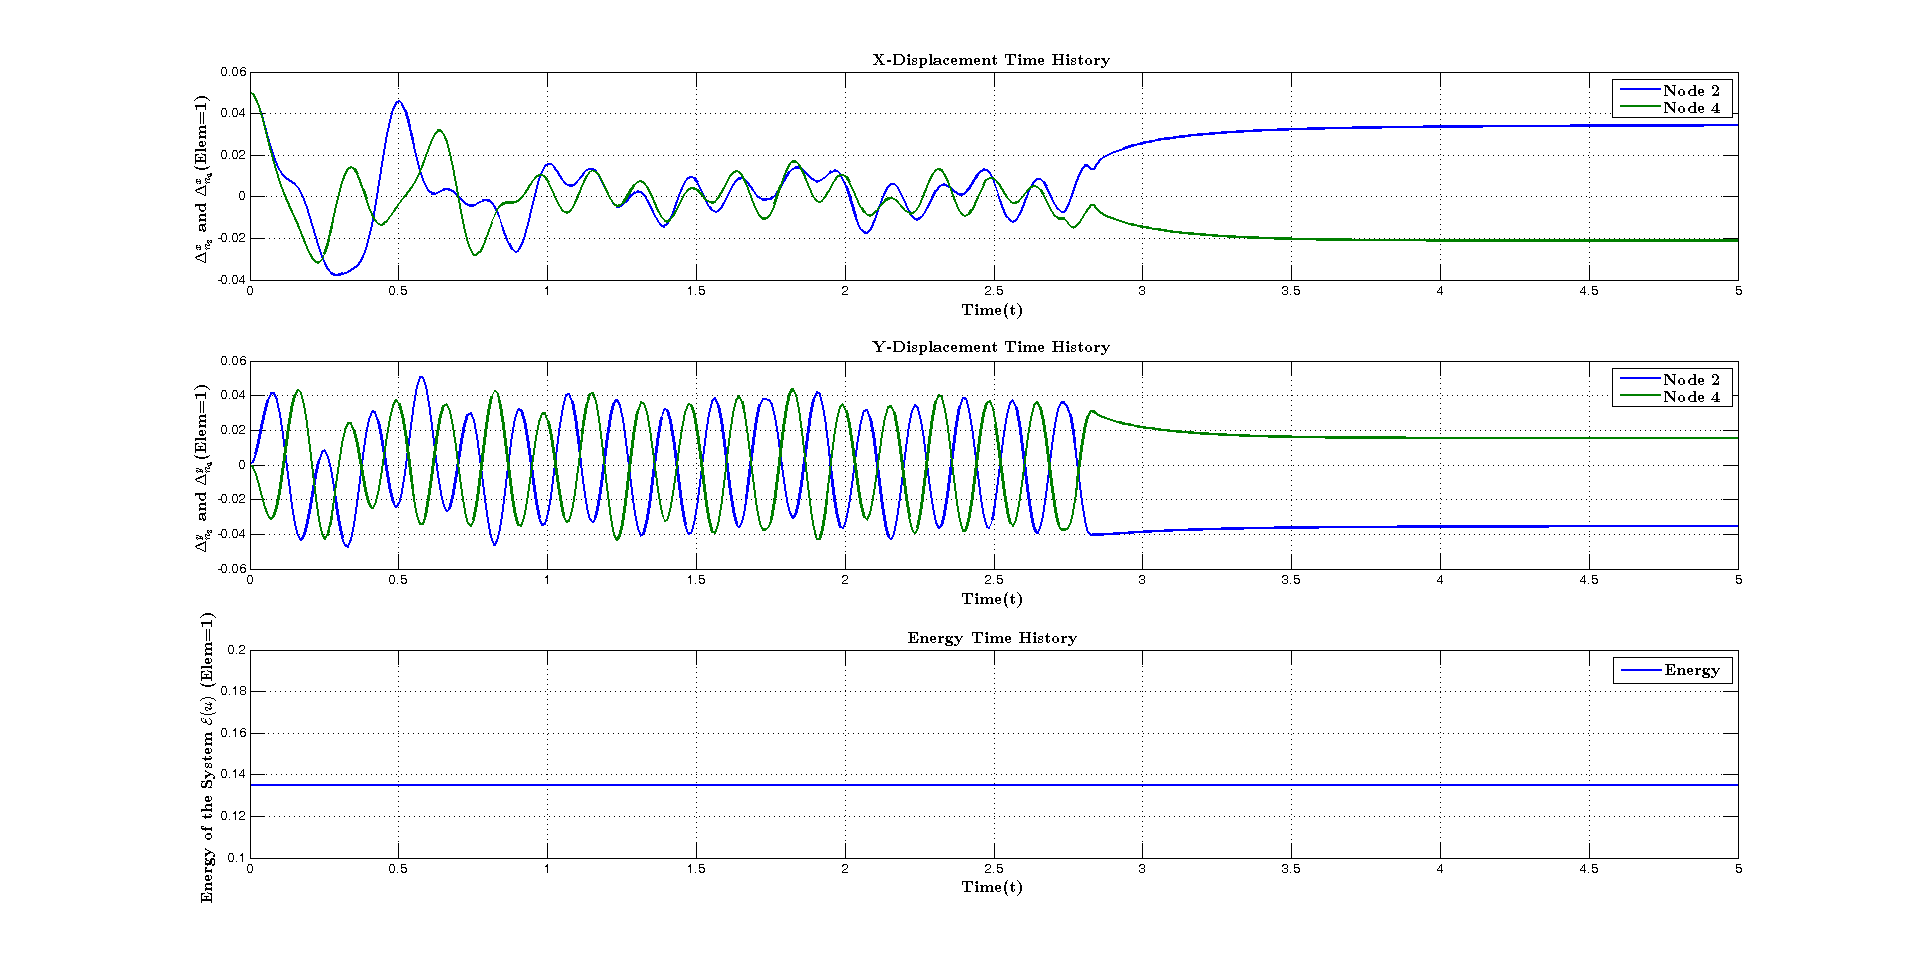
\includegraphics[height=5.5in,width=7in]{Disp_nobf_alphm1_3}
\end{center}\hrule
\item { \bf Comments: } In addition to the comments made in the previous section when alpha is equal to zero, here we note that the response does change significantly. Moreover this response is not unconditionally stable, as $\beta\neq\frac{(1-\alpha)^2}{4}$ and $\gamma\neq\frac{1-2\alpha}{2}$. Note that for this case, and all the subsequent cases when $\alpha = -1/3$ we do not prescribe any upper limit on the number of iterations in the inner loop in Newton-Raphson. This is to observe if there are any time dependent numerical errors which accumulate over several periods to give rise to the divergence as is apparent in the above case. It we calculated only the time-history till $t=2.5s$ it would give us an impression that the algorithm is convergent and well-behaved. However, as can be seen above, this is not the case. 
\newpage 
\item {\bf Stress-Strain Time Histories}
\begin{center}
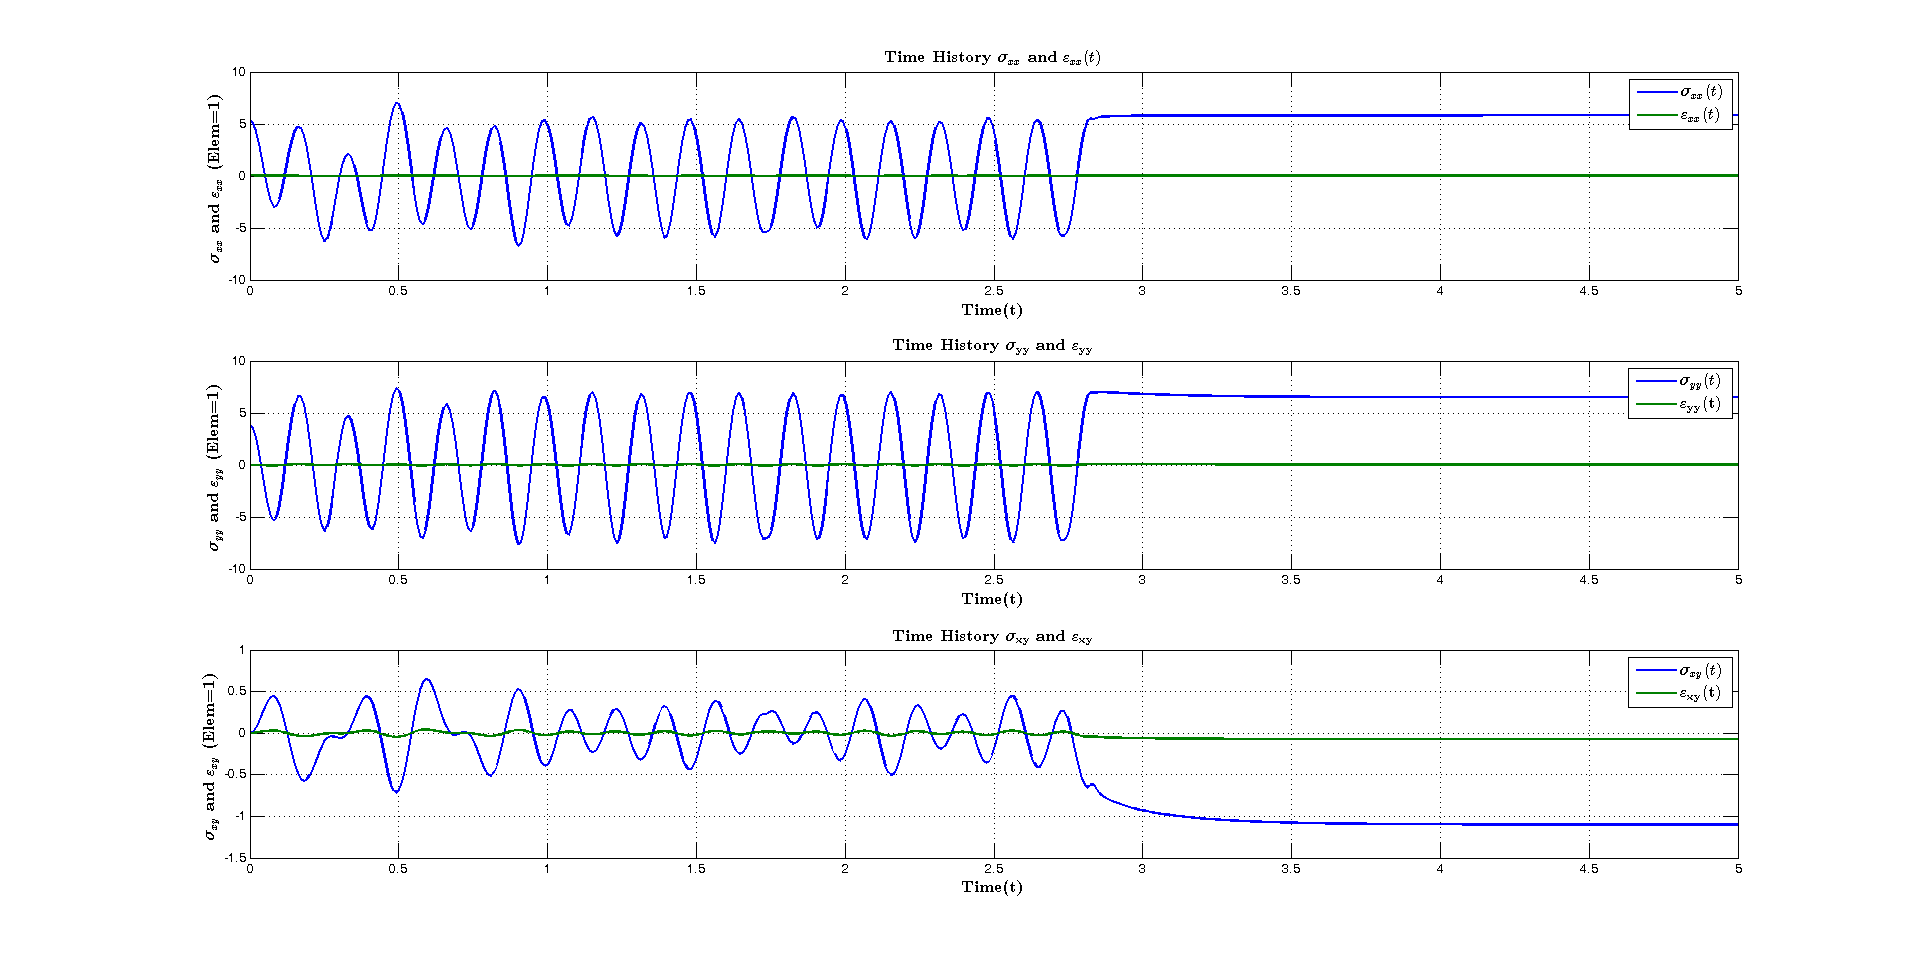
\includegraphics[height=5.5in,width=7in]{Sress_nobf_alphm1_3}
\end{center}\hrule
\item { \bf Comments: } Since we have already concluded from the displacement-time histories, that the algorithm was diverging for the given time step, the above results aren't valid, and moreover reaffirm our observation. 
\end{itemize}
\newpage
For the case when body force is applied we get the following results 
\begin{itemize}
\item {\bf Displacement and Energy Time Histories}
\begin{center}
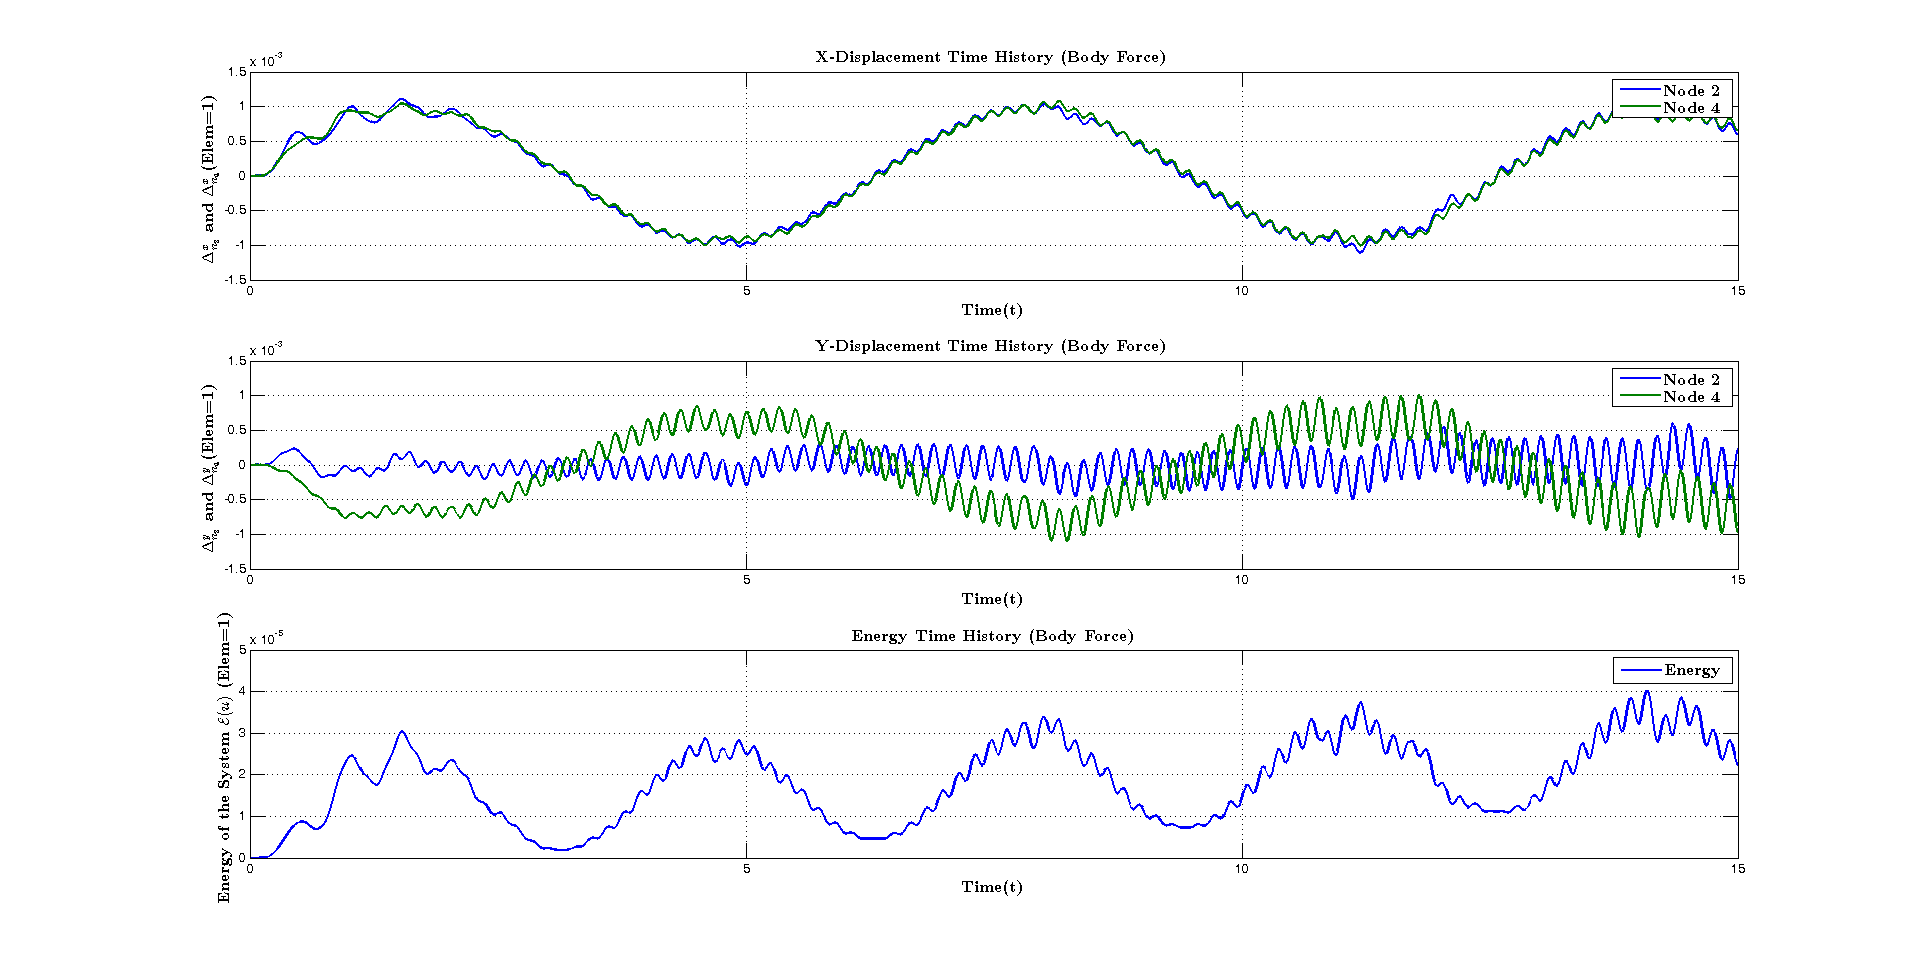
\includegraphics[height=5.5in,width=7in]{Disp_bf}
\end{center}\hrule
\item {\bf Comments: } The nodal displacements follow nearly the same pattern as in the case of the Newmark's method. However the energy, on average, in each cycle is higher than the Newmark's method. The  results, however, are not reliable due to the fact that the algorithm diverges in absence of the body force and hence, computation is done for a smaller time step later in the report.  
\newpage
\item {\bf Stress-Strain Time Histories}
\begin{center}
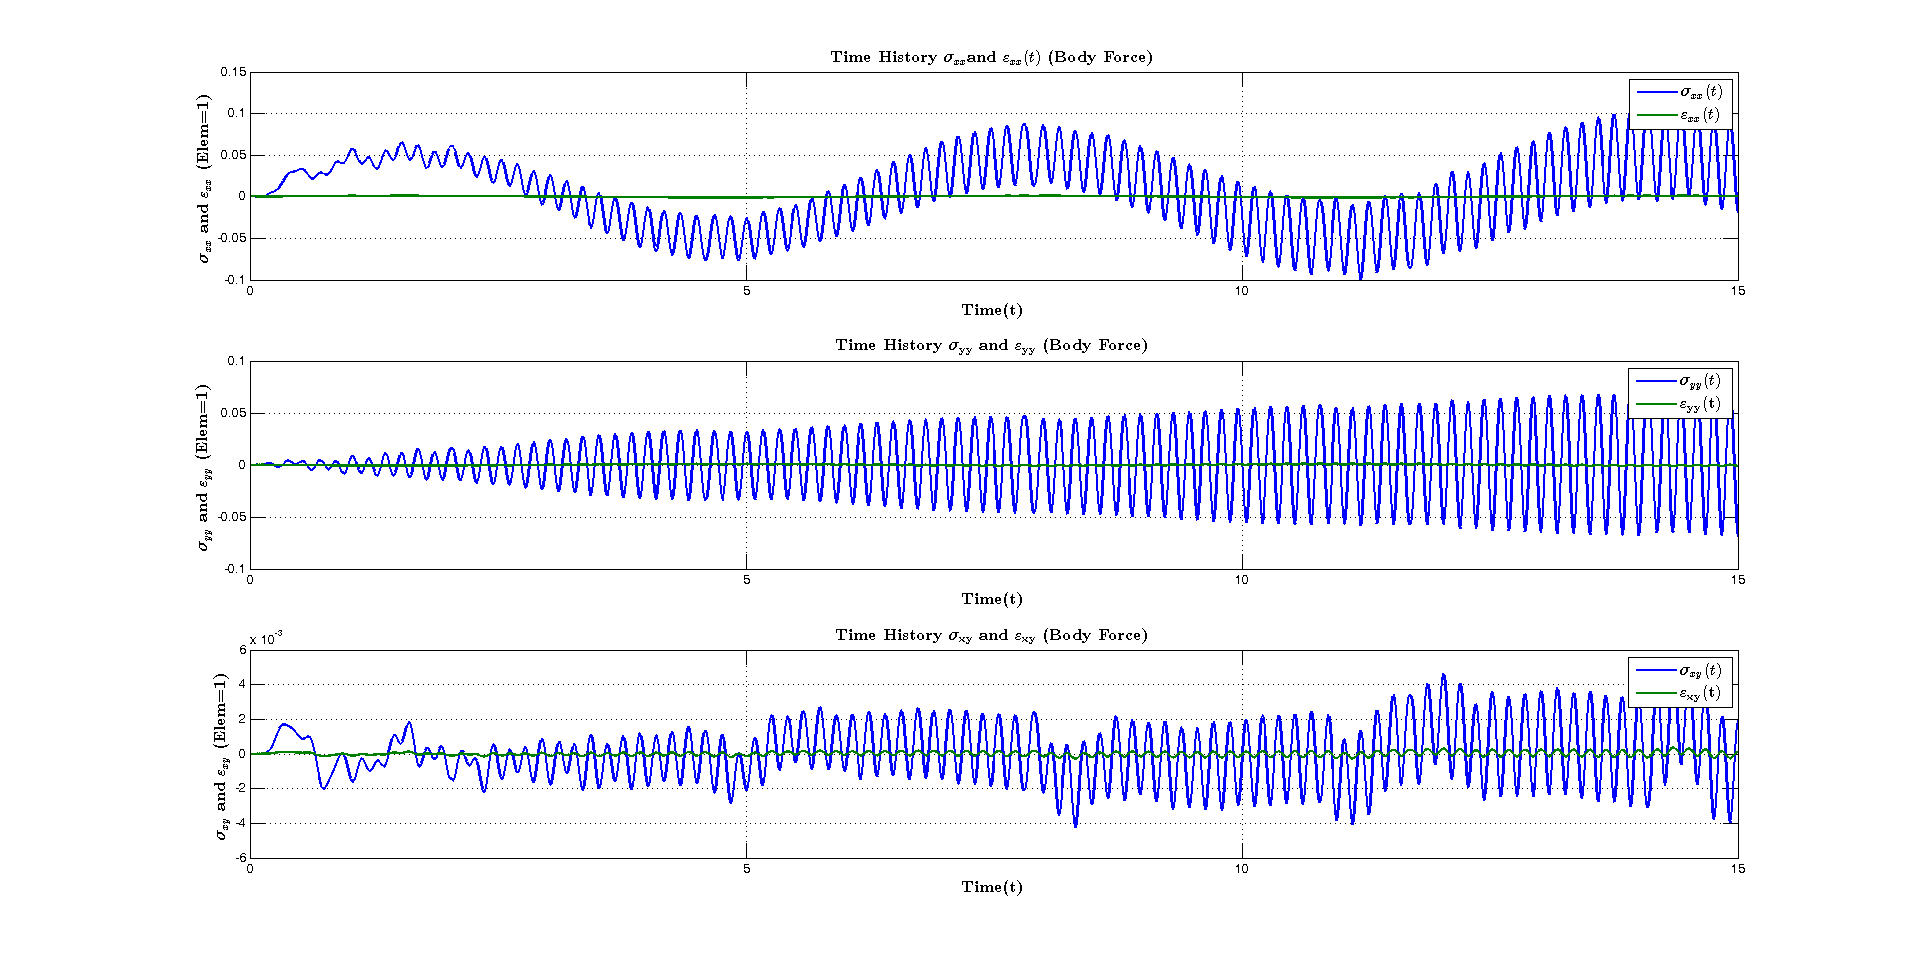
\includegraphics[height=5.5in,width=7in]{Stress_bf}
\end{center} 
\end{itemize}
\hrule
\section*{Appendix: Code Instructions }
The following instructions are applicable in order to run the code. The input file is ($triangtwo.m$)
\begin{itemize}
\item In order to ease the run, there are the following switch cases available to the user (TA):
\begin{itemize}
\item El.Loading: By default this is set to no loading since no external traction is prescribed on the right edge of the domain. 
\item El.bf: This is the body force controlling switch. It is {\bf True} if the body force is to be applied (for Problem 4) and {\bf False} if there is no prescribed body force. 
\item El.type: This is a control for switching between a 1x1 mesh and the 4x4 mesh asked in the midterm. But the calculations corresponding to the 4x4 mesh are not included. 
\end{itemize}
\item For problem 3, switch El.bf to {\bf False} and proceed. Additional controls such as ending time for the time history and corresponding time increment ($\Delta t$) can be controlled in the starting of the input file ($triangtwo.m$)
\item For problem 4, switch El.bf to {\bf True}
\end{itemize}\hrule 
\newpage 
\section*{Results for ($\bf \Delta t=0.001$)}
Some results ($\alpha=-1/3$), for a smaller time increment are shown below for a representative example: 
\begin{itemize}
\item {\bf Displacement and Energy Time Histories}
\begin{center}
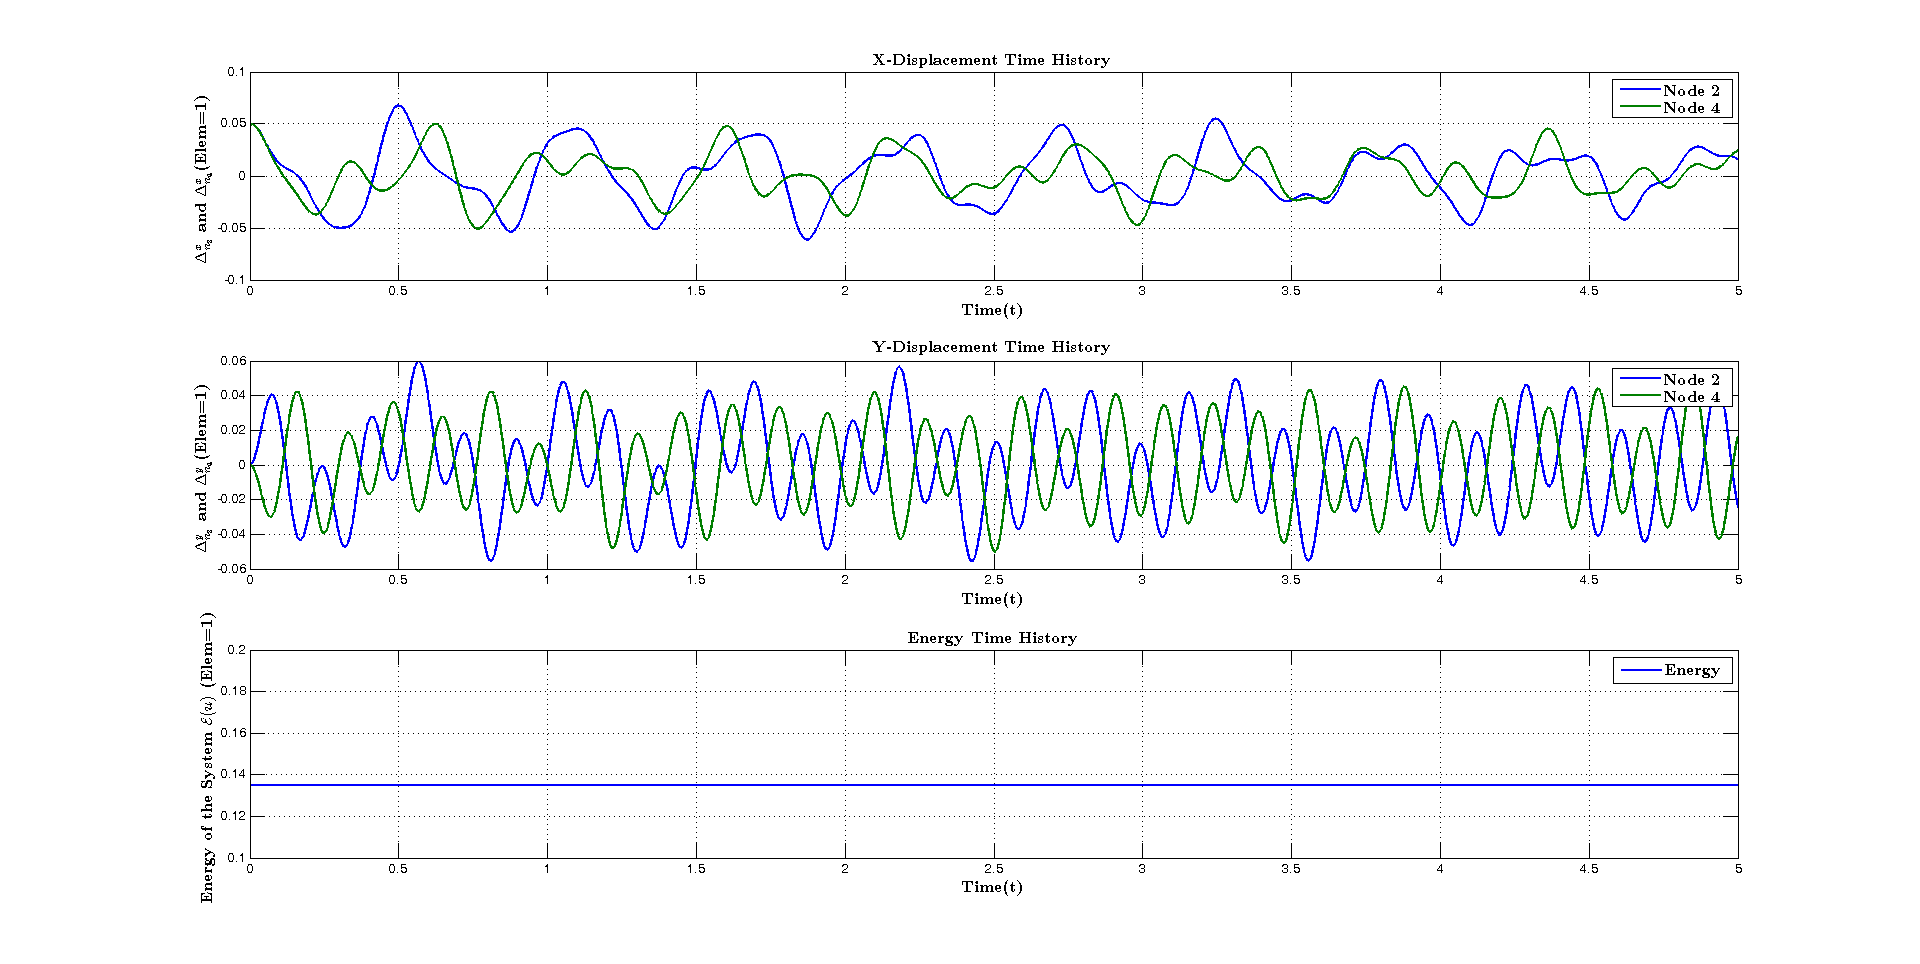
\includegraphics[height=6in,width=6in]{Disp_nobf_alphm1_3_delt_001}
\end{center}
\item {\bf Comments: } It can be seen that the amplification (and consequent divergence), that was observable in the Stress-time histories (and displacements respectively) in the case of $\Delta t = 0.01$, is not there now. A possible reason for this could be that the time increment that we had previously chosen was close to a resonant time period. However it may not be possible to resolve to arbitrarily smaller time increments to numerical precision, and moreover the formulation itself is not unconditionally stable. For nonlinear dynamic applications in general, the time increment and the mesh size cannot be arbitrarily refined independent of each other beyond a point. It is stable, in this case, but may not remain stable for arbitrarily smaller time (and space) increments. \\ 
\hrule
\newpage \item {\bf Stress-Strain Time Histories}
\begin{center}
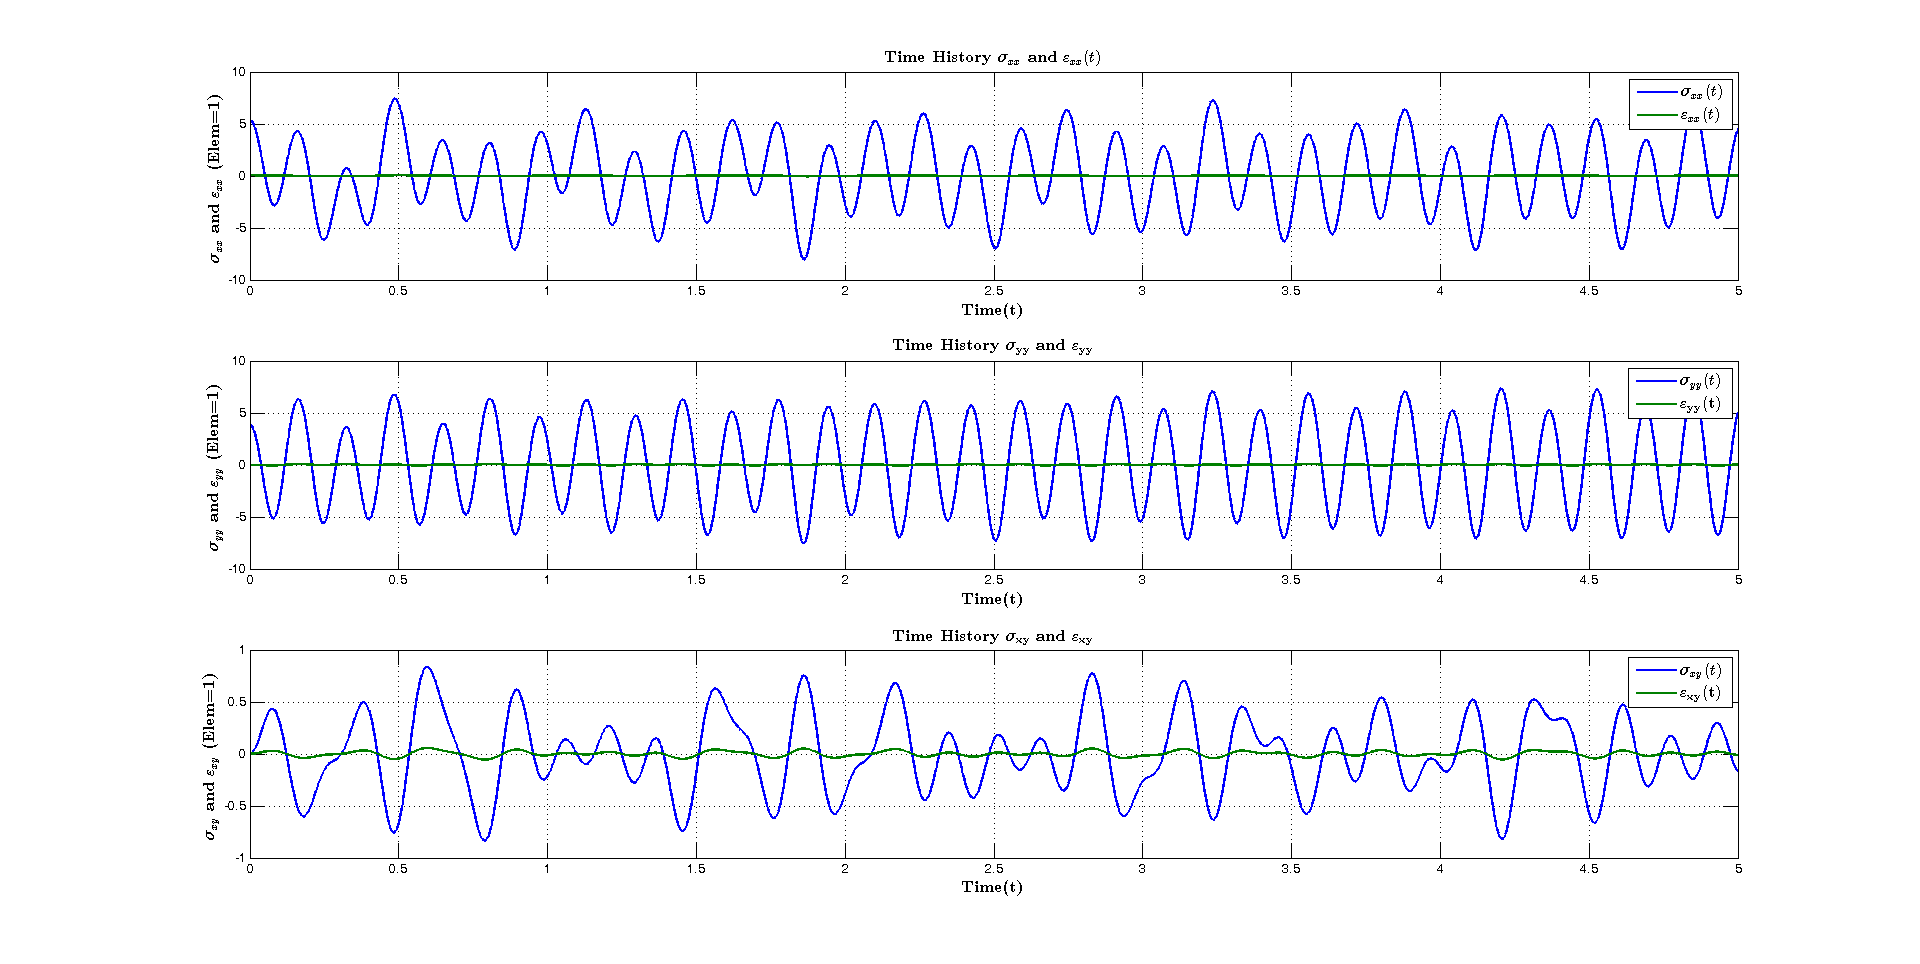
\includegraphics[height=5.5in,width=7in]{Stress_nobf_alphm1_3_delt_2}
\end{center}
\hrule
\item {\bf Comments: } 
The Stress-Strain time histories, in this case are convergence as opposed to the previous formulation. Note that in both the cases, i.e. $\Delta t = 0.01s$ and $\Delta t = 0.001s$ the restriction on the maximum number of iterations was averted to forsee any instability to the numerical errors which creeps overtime and thus causes divergence. And this was verified with the plots.
\end{itemize} 
\newpage
The corresponding results for $\Delta t = 0.001s$ and body force are as follows: 
\begin{itemize}
\item {\bf Displacement and Energy Time Histories}
\begin{center}
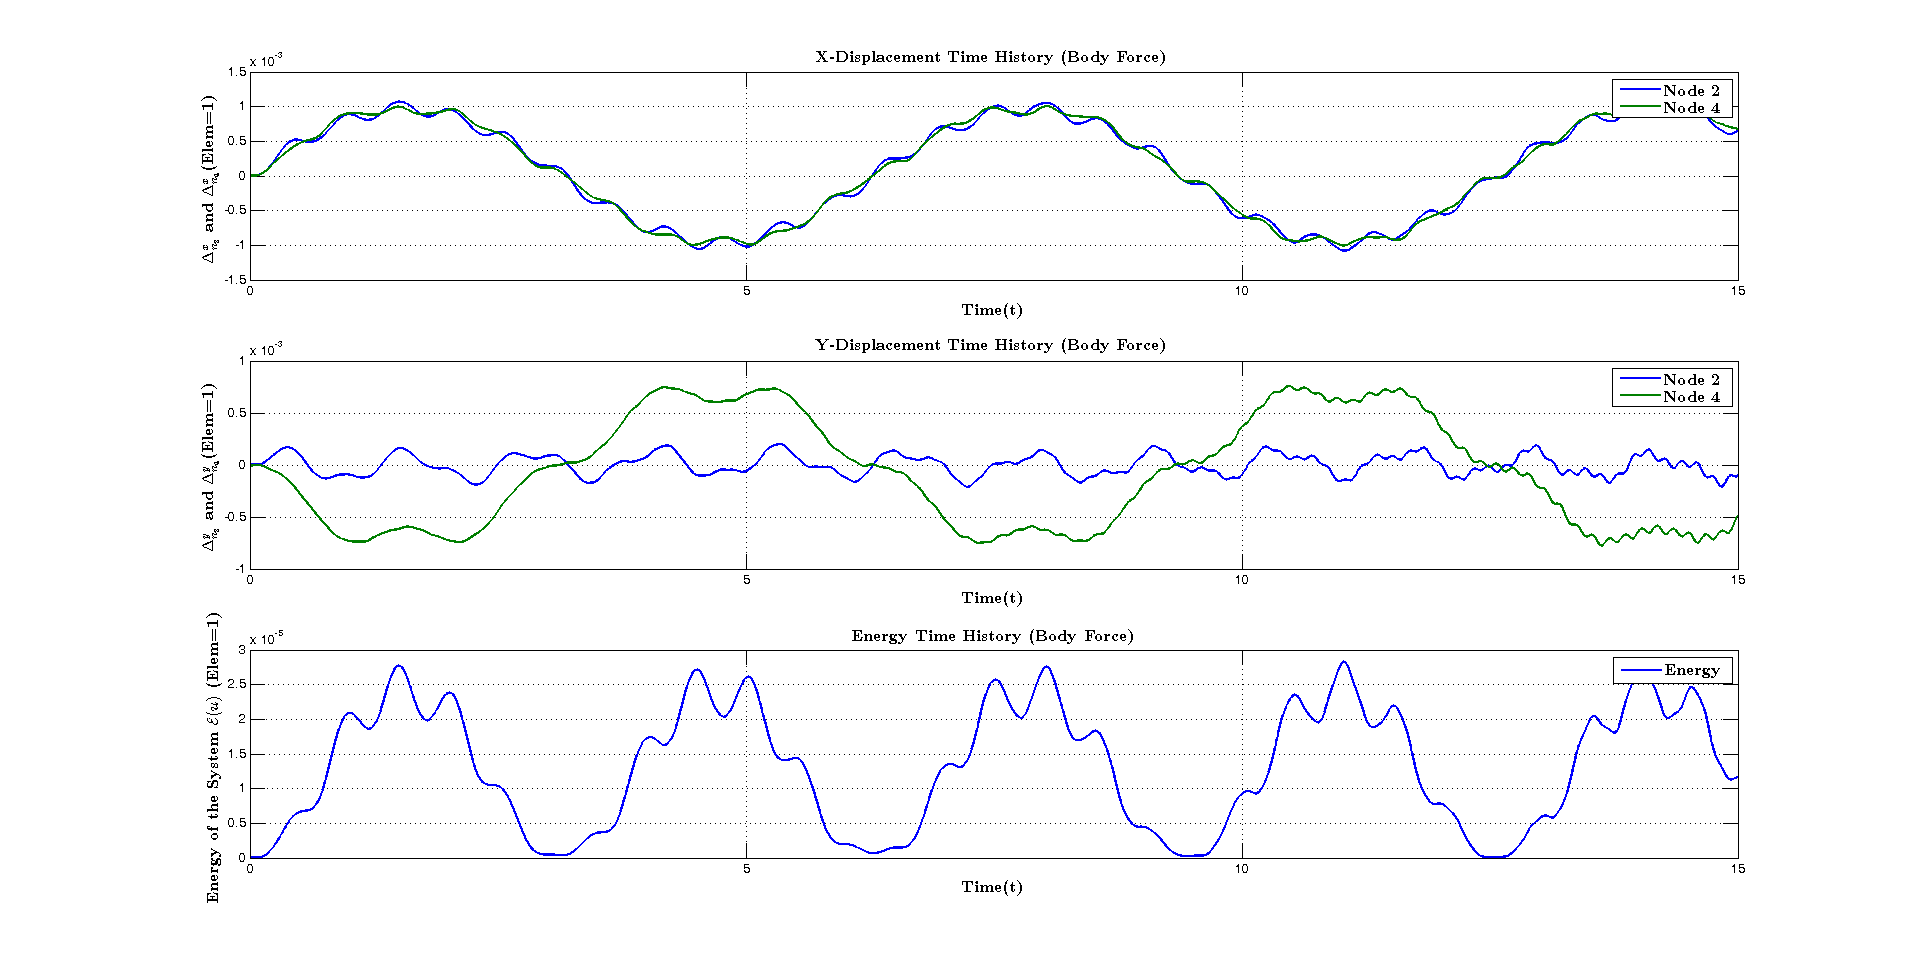
\includegraphics[height=5.5in,width=7in]{Disp_bf_alphm1_3_delt_2}
\end{center}\hrule
\item {\bf Comments: } The displacement, energy and stress-strain time histories reaffirm convergent behavior which was absent in case of smaller time step. 
\newpage
\end{itemize}
\section*{Results for $\bf\Delta t = 0.001s$ and $\bf t_f = 15s$}
Several representative results are presented below to verify the accumulation of numerical errors towards the end of the end of the time history. For the case when no body force is applied, we have: 
\begin{itemize}
\item { \bf Displacement and Energy Time Histories :}
\begin{center}
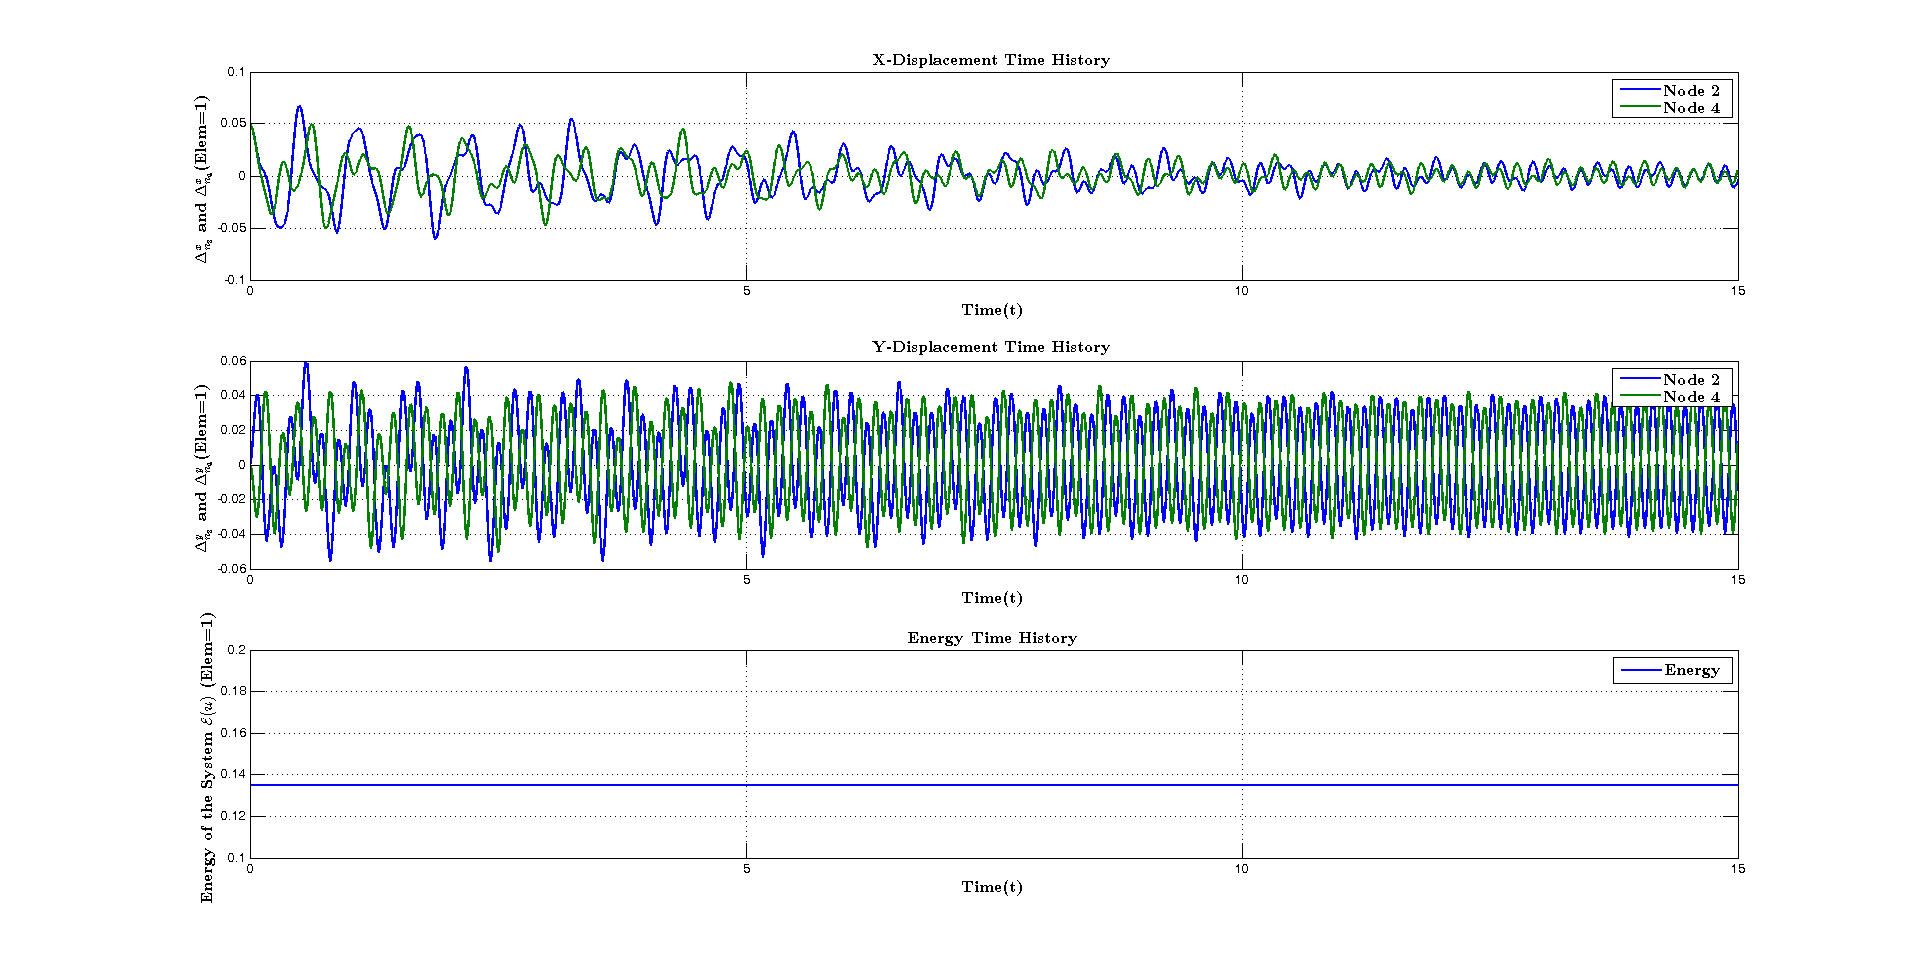
\includegraphics[height=5.5in,width=7in]{Disp_nobf_alphm1_3_delt_2_tf}
\end{center}\hrule
\newpage
\item { \bf Stress and Strain Time Histories :}
\begin{center}
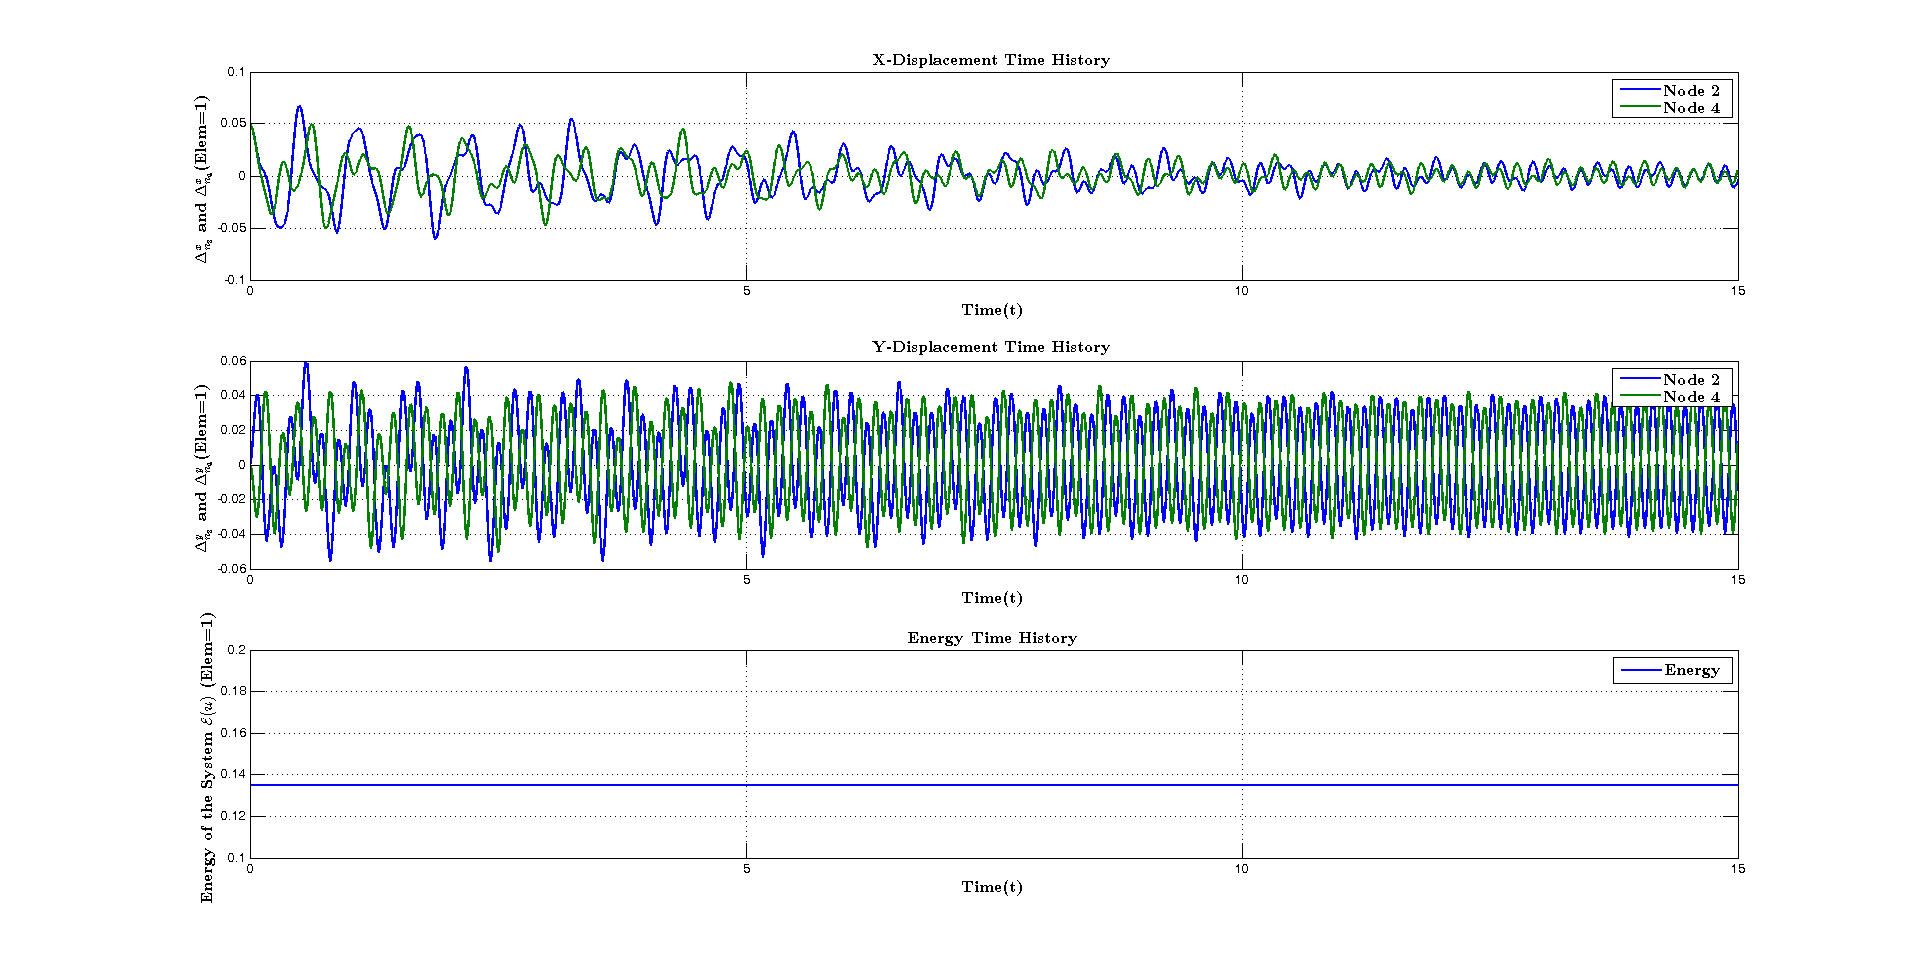
\includegraphics[height=5.5in,width=7in]{Stress_nobf_alphm1_3_delt_2_tf}
\end{center}\hrule
\end{itemize}
\newpage
For the case when body force is applied, we get the following results
\begin{itemize}
\item { \bf Displacement and Energy Time Histories :}
\begin{center}
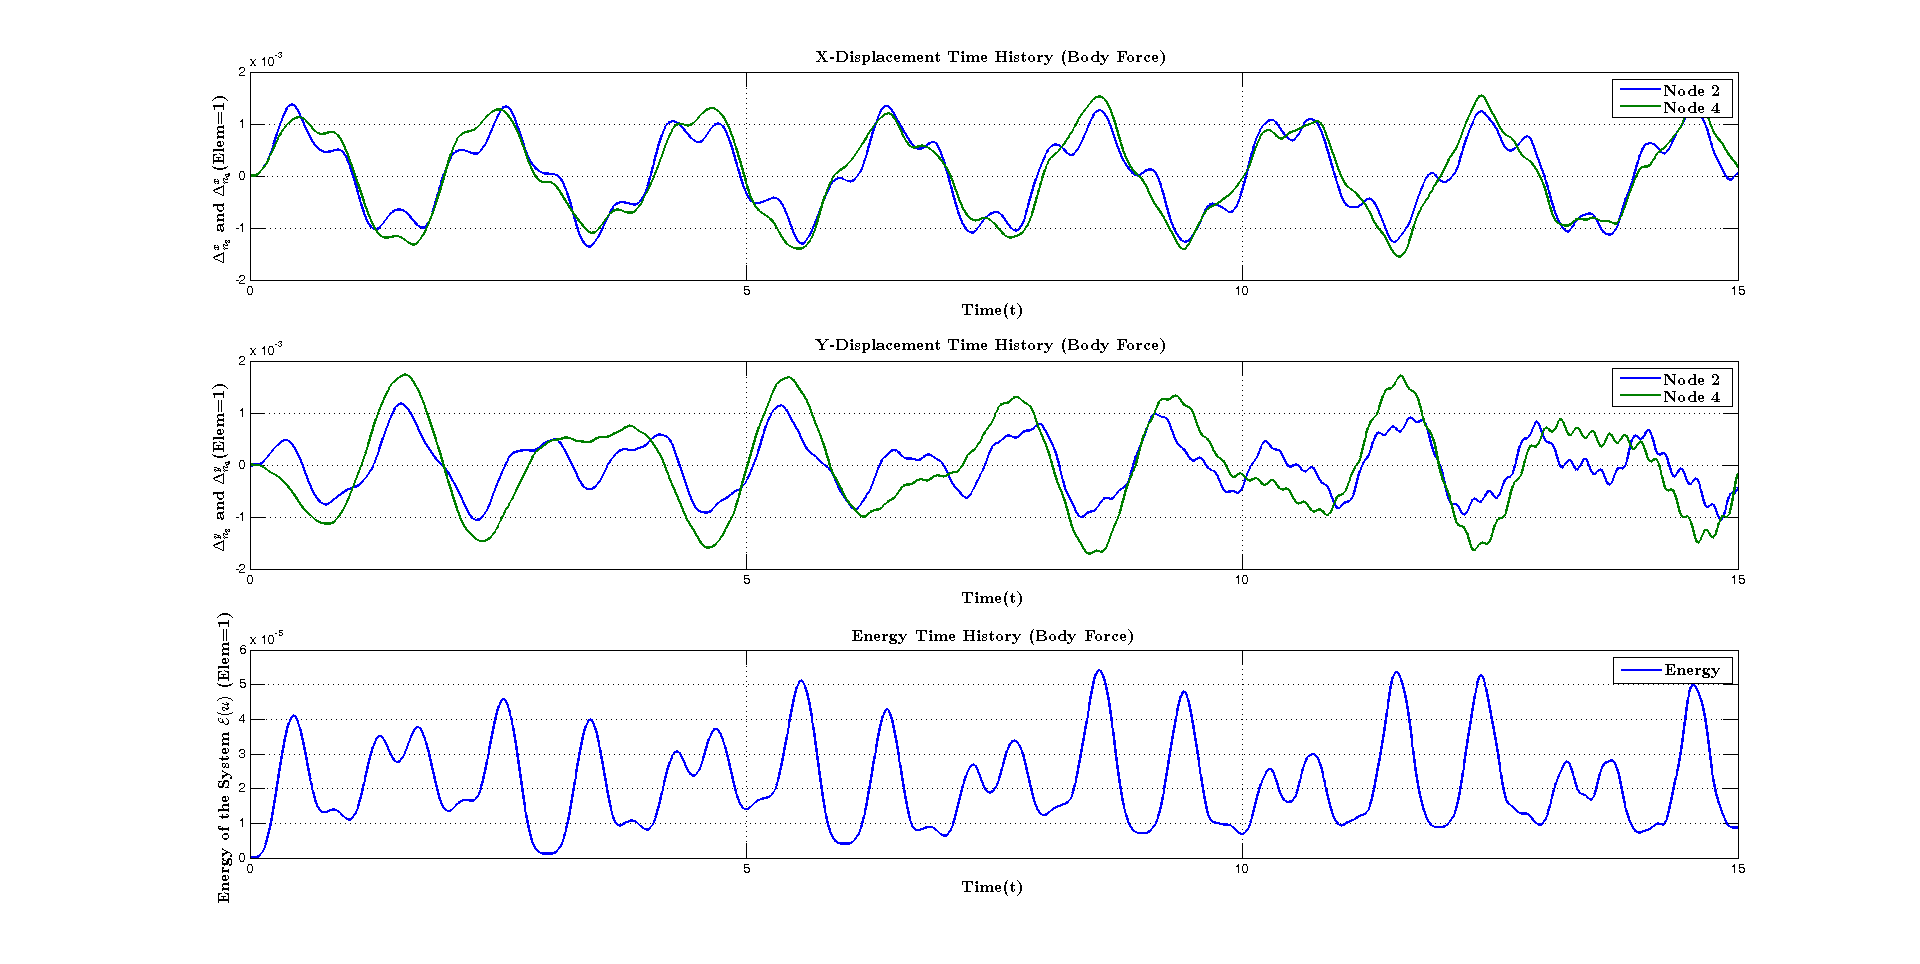
\includegraphics[height=5.5in,width=7in]{Disp_bf_alphm1_3_delt_2_tf}
\end{center}\hrule
\newpage
\item { \bf Stress and Strain Time Histories :}
\begin{center}
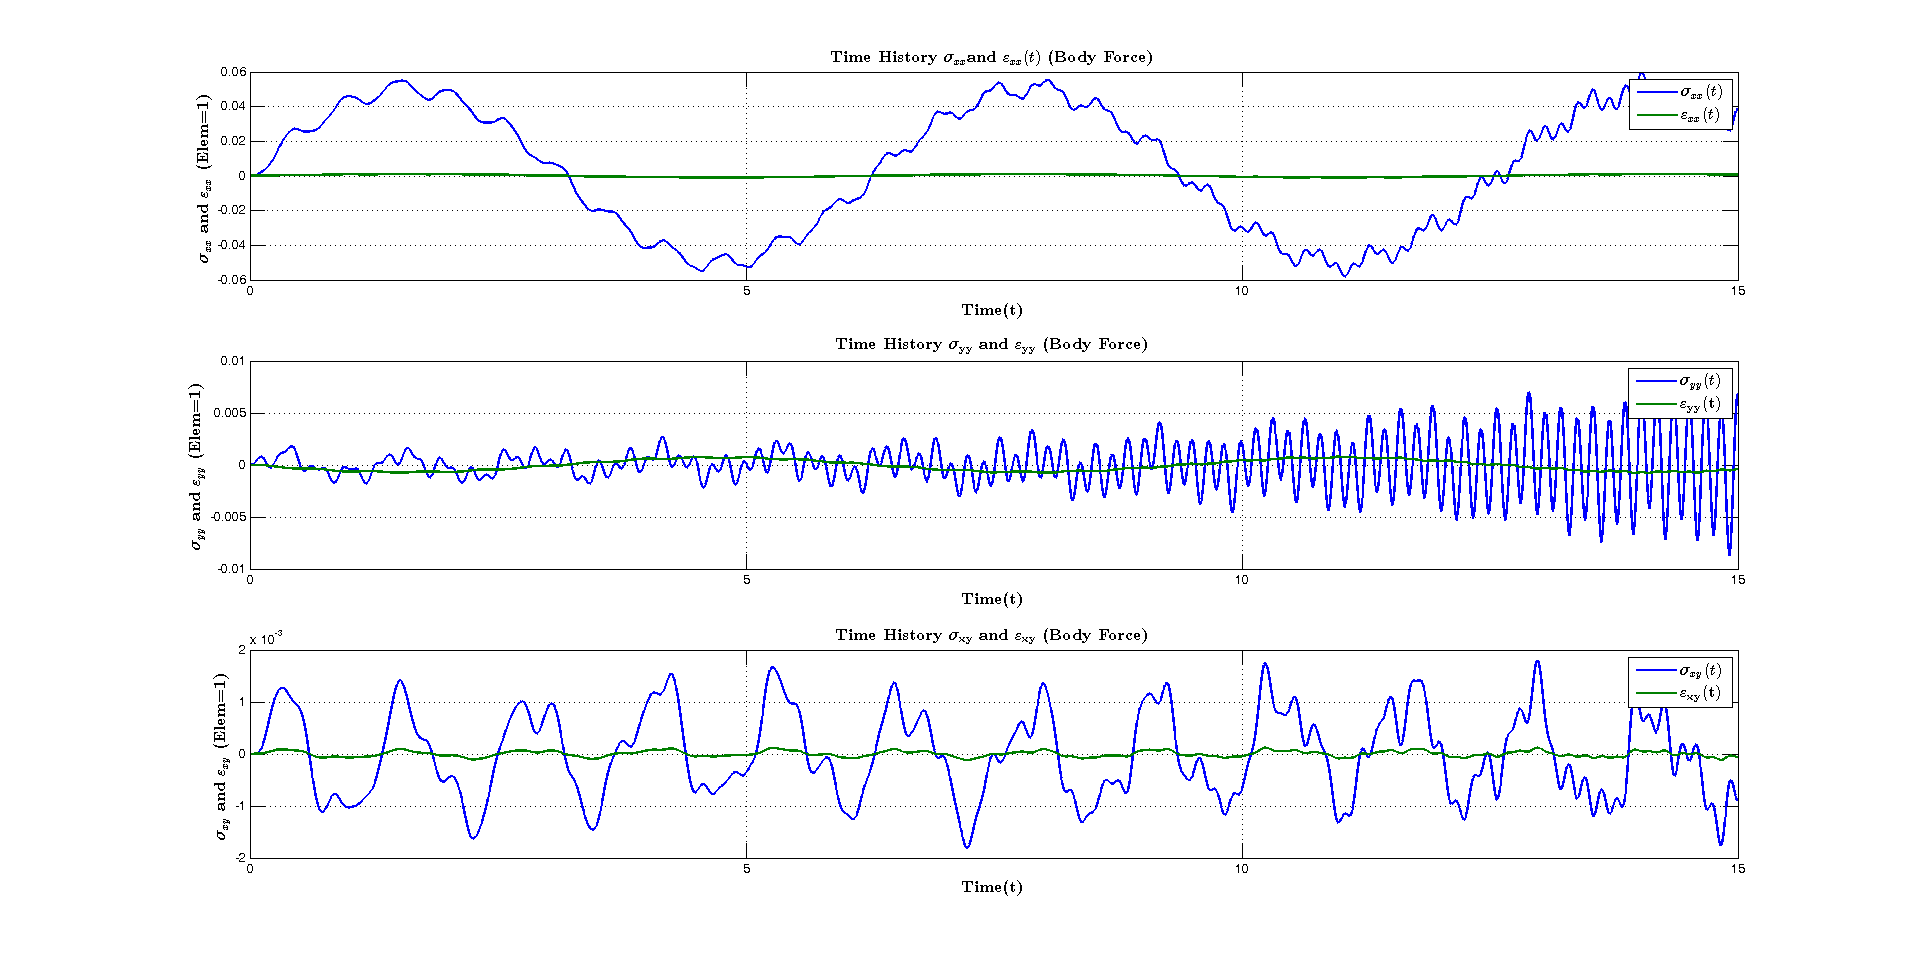
\includegraphics[height=5.5in,width=7in]{Stress_bf_alphm1_3_delt_2_tf}
\end{center}\hrule
\end{itemize}
\subsection*{Conclusion: }
It is plain from the plots above that there is a gradual amplification in all the quantities (due to the accumulating numerical errors). Since the algorithm is not unconditionally stable, it is possible that after a sufficiently long time the results would diverge. And same goes for smaller and smaller time increments (though it is not possible to make it arbitrarily small without refining the mesh). An alternative to this can be the generalized alpha method where the $\beta$ and $\gamma$ values are a function of the dimensionless parameter $\alpha$.\\ \hrule \hrule \hrule 
\end{document}